\chapter{The Semantics of FOL}\label{ch:FOLSemantics}

Recall that in TFL, we had the notion of a \emph{valuation}: an assignment of truth values to atomic sentences.  We then gave a semantics that allowed us to compute the truth value of an arbitrarily complex TFL sentence on any given valuation.  Finally, we used this notion of truth-on-a-valuation to define various logical concepts, like equivalence and entailment.

In this chapter we will do something very similar for FOL, except that the notion of a valuation now gets replaced by the more complex notion of an \emph{interpretation}.  We'll first have to see what an FOL interpretation is, and then learn how to compute the truth values of arbitrarily complex FOL sentences in a given interpretation.  With that in hand, we can then again define logical concepts --- like logical entailment, or validity --- for FOL.

Ultimately, we'll be able to use this machinery to show that a given FOL argument is \emph{not} valid, by giving an interpretation that makes its premises true and its conclusion false.  For reasons that will emerge in this chapter, we won't use interpretations to show that arguments \emph{are} valid.  We will use the natural deduction proofs we learned in chapter \ref{ch:NDFOL} to do this.


\section{Predicates and their Extensions}

The connectives of TFL are all truth-functional, and consequently, TFL only cares about what truth-values sentences have. We can assign a truth value to a sentence \emph{directly}, via a valuation that just stipulates that the sentence `$P$', for example, is to have the value \emph{true}. Alternatively, we can do it \emph{indirectly}, by offering a symbolization key, e.g.:
	\begin{ekey}
		\item[P] Big Ben is in London
	\end{ekey}
This stipulates that the TFL sentence `$P$' is to have the same truth value as the English sentence `Big Ben is in London' (which, as it happens, is true).  But no further aspect of the meaning of the English sentence carries over to TFL.


FOL is similarly impoverished as regards meaning. It goes beyond mere truth values, because it  allows us to split atomic sentences into their parts, consisting of terms and predicates.  A term is a word that refers to a particular object, and a predicate is a word that is \emph{true of} objects.  But FOL doesn't care about any other aspect of predicate's meaning besides what objects it's true of, or any other aspect of a term's meaning besides what it refers to.  For example, when we provide a symbolization key for some FOL predicate, such as:
	\begin{ekey}
		\item[S] \blank\ is a US state.
	\end{ekey}
this isn't intended to suggest that our FOL predicate `$S$' carries the same \emph{meaning} as the English predicate.  It simply tells us that the FOL predicate is to be \emph{true of} exactly those things that the English predicate `\blank \ is a US state' is true of.

Alternatively, we can stipulate what objects a predicate is true of \emph{directly}, by just listing those objects.  So we might stipulate that `$S$' is to be true of: Alabama, Alaska, Arizona, \ldots and so on, listing all 50 states.  This is a perfectly legitimate interpretation of an FOL predicate, because, again, all we care about is what objects it's true of, and our stipulation settles this.  The things a predicate is true of comprise the \define{extension} of the predicate.  FOL is said to be an  \define{extensional language} because it doesn't care about any aspect of a predicate's meaning besides its extension.

Our stipulations about predicate extensions can be as arbitrary as we like. For example, we could stipulate that `$H$' should have an extension consisting of the following objects:
	\begin{ekey}
		\item[H] Barack Obama, the number $\pi$, the play \emph{Hamlet}
	\end{ekey}
It doesn't matter that these objects have nothing in common, they still form a perfectly good predicate extension.  Suppose we add the following names to our symbolization key:
	\begin{ekey}
		\item[b] Usain Bolt
		\item[o] Barack Obama
		\item[p] the number $\pi$
	\end{ekey}
Together, these stipulations then settle the truth value of any atomic FOL sentence formed from the predicate `$H$' and the names `$d$', `$o$', and `$p$': the sentences `$Ho$' and `$Hp$' will both be true on this interpretation, because Obama and $\pi$ are in the predicate's extension, but `$Hb$' will be false, because Usain Bolt is not one of the objects `$H$' is true of.

%\section{Many-place predicates}

\paragraph{Many-Place Predicates} Things get slightly more complicated when we move from one-place predicates to two-place predicates. Consider a symbolization key like:
	\begin{ekey}
		\item[L] \blank loves \blank
	\end{ekey}
This key should be read as saying something like:

	\begin{earg}
		\item[] `$L$' is true of $x$ and $y$ (in that order) iff x loves y.
	\end{earg}
The qualifier ``in that order'' is very important here.  Since $x$ might love $y$ without $y$ also loving $x$, a two-place predicate like this can apply to a pair of objects in one order but not another.

How should a direct stipulation of the extension of a two-place predicate like this look? This is a bit tricky. If we just \emph{list} objects that `$L$' applies to, we won't know which of the objects are the lovers and which are the objects they love.  A simple list would in other words give us no way to indicate the order in which the predicate holds of objects.


To deal wit this, we instead let two-place predicates be true of \emph{pairs} of objects. We could for example stipulate that `$R$' is to be true of, and only of, the following pairs of objects, indicated with angle brackets:
	\begin{center}
	\begin{itemize}
		\item[$R:$] \ntuple{Lenin, Marx}\\
		\ntuple{Heidegger, Sartre}\\
		\ntuple{Sartre, Heidegger}\\
		\ntuple{Marx, Marx}
	\end{itemize}
	\end{center}
The angle-brackets tell us in what order the predicate $R$ applies to the objects: the first object between the brackets always corresponds to the first argument slot in the predicate, and the second object corresponds to the second argument slot. Suppose, for example, that we add the following stipulations for names:
	\begin{ekey}
		\item[l] Lenin
		\item[m] Marx
		\item[h] Heidegger
		\item[s] Sartre
	\end{ekey}
Then `$Rlm$' will be true, since the pair \ntuple{Lenin, Marx} is the extension of `$R$'. But `$Rml$' will be false, since \ntuple{Marx, Lenin} is not in the extension of `$R$'. However, both `$Rhs$' and `$Rsh$' will be true, since both \ntuple{Heidegger, Sartre} and \ntuple{Sartre, Heidegger} are on our list of pairs, and $Rmm$ will also be true, since the pair \ntuple{Marx, Marx} is in $R$'s extension.

If we were dealing with a three-place predicate, its extension would consist not of \emph{pairs} of objects, but of ordered \emph{triples} of objects, like \ntuple{Heiddegger, Marx, Sartre}.  And a four-place predicate would have ordered \emph{quadruples} of objects in its extension, a five-place predicate would have ordered \emph{quintuples}, and so on.  In general, we call ordered things like these \define{Tuples}.  So the extension of a many-place predicate can be specified by giving a list of tuples: either of pairs, or of triples, or of quadruples etc. depending on whether we're dealing with a two-, three-, or four-place predicate.

%To make these ideas more precise, we would need to develop some very elementary \emph{set theory}. Set theory has formal apparatus which allows us to deal with extensions, ordered pairs, and so forth. However, set theory is not covered in this book. So I shall leave these ideas at an imprecise level. I hope that the general idea is clear enough.


% \section{Semantics for identity}
%
%\paragraph{The Identity Predicate} Lastly, we have identity, which receives special treatment in FOL.  As we've seen, we write it a bit differently from other two-place predicates: `$x=y$' instead of `$Ixy$' (for example). More important, though, is that its interpretation is fixed, once and for all.  The way to determine the truth value of an identity statement is very simple: $\meta{a} = \meta{b}$ is true if \meta{a} and \meta{b} refer to the same object, and false otherwise.
%
%So given our stipulations above, `$m = m$' and `$w=w$' are, for example, both true, whereas `$w=m$' or `$l=s$' are false.  It's important to notice, though, that identity statements involving two different names can be still be true if the two names refer to the same object.  For example, if we had the following symbolization key:
%	\begin{ekey}
%		\item[l] Lady Gaga
%		\item[c] Kurt Cobain
%		\item[g] Lady Gaga
%	\end{ekey}
%then `$l=g$' and `$g=l$' would both be true despite involving different names.  Having two names for the same object isn't that unusual, and in fact happens all the time when people have nicknames, pseudonyms, or stage names: `Stefani Germanotta' and `Lady Gaga' refer to the same person, and so do `Jay-Z' and `Shawn Carter', for example.



%
%If two names refer to the same object, then swapping one name for another will not change the truth value of any sentence. So, in particular, if `$a$' and `$b$' name the same object, then all of the following will be true:\label{model.nonidentity}
%	\begin{align*}
%	 	Aa &\eiff Ab \\
%	 	Ba &\eiff Bb\\
%		Raa &\eiff Rbb\\
%		Raa & \eiff Rab\\
%		Rca &\eiff Rcb\\
%		\forall x Rxa &\eiff \forall x Rxb
%	\end{align*}
%Some philosophers have believed the reverse of this claim. That is, they have believed that when exactly the same sentences (not containing `$=$') are true of $a$ and $b$, then $a$ and $b$ are the very same object. This is a highly controversial philosophical claim---sometimes called the \emph{identity of indiscernibles}---and our logic will not subscribe to it. So we allow that exactly the same things might be true of two \emph{distinct} objects.
%
%To bring this out, consider the following interpretation:
%	\begin{ebullet}
%		\item[\text{domain}:] P.D.\ Magnus, Tim Button
%		\item[$a$:] P.D.\ Magnus
%		\item[$b$:] Tim Button
%		\item For every primitive predicate we care to consider, that predicate is true of \emph{nothing}.
%	\end{ebullet}
%Suppose `$A$' is a one-place predicate; then `$Aa$' is false and `$Ab$' is false, so `$Aa \eiff Ab$' is true. Similarly, if `$R$' is a two-place predicate, then `$Raa$' is false and `$Rab$' is false, so that `$Raa \eiff Rab$' is true. And so it goes: every atomic sentence not involving `$=$' is false, so every biconditional linking such sentences is true. For all that, Tim Button and P.D.\ Magnus are two distinct people, not one and the same!

\section{FOL Interpretations}\label{s:FOLInterpretations}


We defined a \emph{valuation} of a sentence \meta{\varphi} (or collection of sentences) of TFL to be an assignment of truth values to all the atomic sentences contained in \meta{\varphi} (or the collection). In FOL, the role of a valuation will be played by an \define{Interpretation}.  FOL interpretations are more complex than TFL valuations, because they have  \emph{three} components:
\factoidbox{
An \define{FOL Interpretation} of a sentence \meta{\varphi}  (or of a collection of sentences \texttt{C}, e.g. an argument) consist of:
	\begin{enumerate}
		\item A specification of a \define{domain} containing at least one object
		\item For each name in \meta{\varphi} (or in $\texttt{C}$), an assignment of exactly one object in the domain.  This object is the name's \define{referent}.
		\item For each predicate in \meta{\varphi} (or in \texttt{C}), a specification of what objects in the domain (if any), and in what order, that predicate is  true of.  This constitutes the predicate's \define{Extension}.\footnote{So notice that a predicate can have an empty extension, in which case it it isn't true of any objects in the domain.  By contrast, we don't allow ``empty names'' that lack a referent.}
	\end{enumerate}}

Symbolization keys like those we used in chapter \ref{ch:FOLSymbolization} consequently give us one convenient way to present an interpretation.  For example, the following counts as one possible FOL interpretation of `$(Lw \land Tw)$':
	\begin{ekey}
		\item[\text{Domain}] people
		\item[w] Wittgenstein
		\item[L] \blank\ is a logician
		\item[T]\blank\ is a school teacher
	\end{ekey}
This has all three components: (i) a specification of a domain, (ii) a specification of a referent for every name in `$(Lw \land Tw)$', and (iii) a specification of an extension for every predicate in `$(Lw \land Tw)$'.  The interpretation then determines a truth value for the sentence.  In this case, since Wittgenstein was both a logician and a school teacher, both `$L$' and `$T$' are true of the referent of the name `$w$' on this interpretation, and so `$(Lw \land Tw)$' as a whole is true.

Alternatively, we can specify interpretations by just directly listing the objects that predicates are true of,  as discussed in the previous section.  In fact, as we move on, it will often be convenient to consider fairly abstract interpretations where the domain consists of natural numbers, i.e. positive integers, rather than people, or plants, or other objects. One possible interpretation of `$\exists x(Fx \eand Gx)$', for example, would be the following:\footnote{Although this kind of domain officially consists of just numbers,  we could in principle regard it as consisting of any objects we like --- we're just calling these objects `object 1', `object 2', `object 3' etc. for simplicity.}
	\begin{ekey}
		\item[\text{Domain}] 1, 2, 3
		\item[F]
		\item[G] 1, 3
	\end{ekey}
Here the domain contains the numbers 1, 2, and 3, the predicate `$F$' is true of none of those objects, and `$G$' is true of 1 and 3.  As you can probably guess, `$\exists x(Fx \eand Gx)$' comes out false on this interpretation, since there's no object in the domain of which both `$F$' and `$G$' are true.  We'll look at how to determine truth values more closely in the next two sections.

It will  often be useful to represent directly-specified interpretations \emph{diagramatically}.  Interpretations like the one above that involve only one-place predicates can be represented using a \define{matrix diagram}:
\begin{center}\begin{tabular}{|c|c|c|}
\hline
    &   F   &   G   \\ \hline
1   &   $-$   &   $+$   \\ \hline
2   &   $-$   &   $-$ \\ \hline
3   &   $-$   &   $+$ \\ \hline
\end{tabular}\end{center}
Here we list the objects in the domain on the left, and then put $+$'s and $-$'s under each predicate to indicate which objects that predicate is true of.  If we were also considering some FOL names, we could include those in our matrix diagram by listing each name to the left of whichever object it refers to.

As we discussed in the last section, to directly specify the extension of a \emph{many-place} predicate, we have to give a list of \emph{tuples} of objects, rather than of individual objects, to indicate in what order the predicate holds of the objects.  So for example, if we take the sentence `$\forall xRxx$' which contains the two-place predicate `$R$', one possible interpretation would be the following:
	\begin{ekey}
		\item[\text{Domain}] 1, 2, 3, 4
		\item[R]\ntuple{1, 4}, \ntuple{4,4},  \ntuple{1, 2}, \ntuple{2, 1} \ntuple{1, 3},
	\end{ekey}
To represent interpretations with two-place predicates diagramatically, we can use \define{arrow diagrams} like this:
\begin{center}
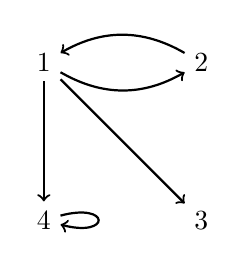
\begin{tikzpicture}
\node (atom1) at (0,2) {1};
\node (atom2) at (2,2) {2};
\node (atom3) at (2,0) {3};
\node (atom4) at (0,0) {4};
\draw[->, thick] (atom1) to[bend right] (atom2);
\draw[->, thick] (atom2) to[bend right] (atom1);
\draw[->, thick] (atom1)--(atom3);
\draw[->, thick] (atom1)--(atom4);
\draw[->, thick] (atom4) to[loop right, looseness=15] (atom4);
\end{tikzpicture}
\end{center}
The arrows represent the order in which `$R$' holds of the objects.  To indicate that 1 bears the relation represented by `$R$' to 4, we draw an arrow from 1 to 4, and to indicate that 4 bears the relation to itself, we draw an arrow that loops from 4 back to 4, and to indicate that 1 bears the relation to 2, and 2 also bears it to 1, we draw two arrows between them, and so on.  So there is one arrow for each pair in the extension of the predicate.

%Or we could give a diagram like this:
%\begin{center}
%\begin{tikzpicture}
%\node (atom1) at (0,2) {1};
%\node (atom2) at (2,2) {2};
%\node (atom3) at (2,0) {3};
%\node (atom4) at (0,0) {4};
%\draw[->, thick] (atom3)--(atom4);
%\draw[->, thick] (atom1) to[loop left, looseness=15] (atom1);
%\draw[->, thick] (atom3) to[loop right, looseness=15] (atom3);
%\draw[<->, thick] (atom1) -- (atom3);
%\end{tikzpicture}
%\end{center}
%to represent the following interpretation:
%	\begin{ekey}
%		\item[\text{Domain}] 1, 2, 3, 4
%		\item[R] \ntuple{1, 1}, \ntuple{1,3},  \ntuple{3, 1}, \ntuple{3, 3}, \ntuple{3,4}
%	\end{ekey}
%As you can probably guess, `$\forall xRxx$' would be false on both of our arrow diagrams, since neither diagram is one on which \emph{every} object bears the relation $R$ to itself.


If we wanted, we could make such arrow diagrams more complex. For example, we could label objects in our diagram with FOL names to indicate which object each name refers to.  To represent the extension of a one-place predicate in an arrow diagram, we could draw a circle around some objects and label the circle with the predicate. And to represent the extensions of multiple two-place predicates in a single arrow diagram, we might use arrows with dashed as opposed to solid lines, or arrows of different colors.



\section{Truth in FOL}\label{s:TruthFOL}

We have introduced interpretations. Our next task is to give a precise account of what it is for an arbitrarily complex FOL sentence to be true or false in a given interpretation. There are three kinds of sentence in FOL: atomic sentences, sentences whose main logical operator is a sentential connective, and lastly, sentences whose main logical operator is a quantifier.  We'll go through each kind in turn.

Our explanation will be completely general, but to make things comprehensible, it will be useful to have a particular interpretation to hand in order to give examples.  Let's use the following as our \emph{go-to interpretation}:
\begin{ekey}
		\item[\text{Domain}] all positive integers
		\item[a] 2
		\item[b] 3
		\item[E] \blank is even
		\item[R] \blank \ is less than \blank
	\end{ekey}
I've here specified the extensions of `$E$' and `$R$' indirectly, using English predicates, because I can't list all the numbers, or pairs of numbers, these are true of.  But the extension of `$E$' contains even numbers $2, 4, 6, 8 \ldots$, and the extension of `$R$' contains the pair \ntuple{2, 3}, as well as \ntuple{2, 4} and \ntuple{2,5} and \ntuple{3, 5}, and indeed every pair \ntuple{x,y} where $x$ is less than $y$.

\paragraph{Truth-Rule for Atomic Sentences} Determining the truth value of an atomic sentence on a given interpretation is fairly straightforward.  The atomic sentence `$Ea$', for example, is true just in case `$E$' is true of the referent of `$a$'.  Given our go-to interpretation, this sentence is true since `$a$' refers to 2, and 2 is indeed an even number.  By contrast, `$Eb$' would be false on our interpretation, because 3, which is the referent of `$b$', is not in the extension of `$E$', since it is not an even number.

Similarly, `$Rab$' is true on our interpretation just in case the referent of `$a$' is less than the referent of `$b$'.  Since 2 is indeed less than 3, `$Rab$' is true.  By contrast, `$Rba$' is not true, because 3 is not less than 2, or to put it another way, the pair \ntuple{3,2} is not in the extension of `$R$' on our interpretation.  Similarly, neither `$Raa$' nor `$Rbb$' are true on our go-to interpretation, since neither 2 nor 3 is less than itself (i.e. the pairs \ntuple{2,2} and \ntuple{3,3} are not in the extension of `$R$').  In general, the truth-rule for atomic sentences is:
	\factoidbox{
		When \meta{R} is an $n$-place predicate and $\meta{c}_1, \meta{c}_{2}, \ldots, \meta{c}_{n}$ are names, the sentence $\meta{R}\meta{c}_{1}\meta{c}_{2}\ldots\meta{c}_{n}$ is true in a given interpretation \textbf{iff} $\meta{R}$ is true of the objects referred to by $\meta{c}_{1}, \meta{c}_{2}, \ldots, \meta{c}_{n}$ (in that order) in that interpretation	}

%There is one additional kind of atomic sentence to consider: those formed by connecting two names with an identity sign.  As already mentioned, determining the truth values of identity statements is straightforward:
%\factoidbox{
%		For any names $\meta{a}$ and $\meta{b}$, the sentence $\meta{a} = \meta{b}$ is true in a given interpretation \textbf{iff}
%		 \meta{a} and \meta{b} refer to very same object in that interpretation
%	}
%So, in our go-to interpretation, `$a = b$' is false, since `$a$' refers to the number 2 and `$b$' to the number 3, and 2 is distinct from 3.  On the other hand, both `$a=a$' and `$b=b$' are true.

\paragraph{Truth-Rules for TFL Connectives} The truth rules governing our truth-functional operators are exactly the same as they were in TFL:

\factoidbox{
$\enot \meta{\varphi}$ is true in a given interpretation \textbf{iff} $\meta{\varphi}$ false in that interpretation\\

$(\meta{\varphi} \eand \meta{\psi})$ is true in a given interpretation \textbf{iff} both $\meta{\varphi}$ and $\meta{\psi}$ are true in that interpretation\\

$(\meta{\varphi} \eor \meta{\psi})$ is true in a given interpretation \textbf{iff} either $\meta{\varphi}$ or $\meta{\psi}$ is true in that interpretation\\


$(\meta{\varphi} \eif \meta{\psi})$ is true in a given interpretation \textbf{iff} either $\meta{\varphi}$ is false or $\meta{\psi}$ is true in that interpretation.\footnote{This means that $(\meta{\varphi} \eif \meta{\psi})$ is false if $\meta{\varphi}$ is true and  $\meta{\psi}$ is false, and true otherwise. }\\

$(\meta{\varphi} \eiff \meta{\psi})$ is true in a given interpretation \textbf{iff} $\meta{\varphi}$ has the same truth value as $\meta{\psi}$ in that interpretation
	}
This  is equivalent to the information conveyed by the characteristic truth tables for the connectives; it's just presented in words here rather than truth tables.   Some examples will help to illustrate the idea (make sure you understand them!). On our go-to interpretation:
	\begin{earg}
		\item[\textbullet]  `$\enot Raa$' is true because 2 is not less than itself
		\item[\textbullet] `$Rab \eand Ea$' is true because both conjuncts are true
		\item[\textbullet] `$Rab \eand Eb$' is false because, although `$Rab$' is true, `$Eb$' is false
		\item[\textbullet] `$Eb \eif \enot Rba$' is true because `$Eb$' is false.
		%\item[\textbullet] `$a=b \eor Ea$' is true because although `$a=b$' is false, `$Ea$' is true
		%\item[\textbullet] `$a \neq b \rightarrow Rba$' is false because the antecedent is true and the consequent is false
		\end{earg}

\section{Truth-Rules for Quantified Sentences}\label{s:TruthQuantifiedSentences}

The big innovation in FOL is the use of \emph{quantifiers}. And specifying the truth conditions for quantified sentences turns out to be a little tricky.  If we only look at simple cases things are pretty straightforward.  We can say that `$\exists xEx$' is true iff `$E$' is true of at least one object in the domain, and  `$\forall xEx$' is true iff `$E$' is true of every object in the domain.  So on our go-to interpretation, `$\exists xEx$' comes out true, and `$\forall xEx$' comes out false.


But what about a more complex sentence like `$\forall x(Ex \rightarrow Rxb)$'?  This has a universal quantifier as its main operator, so we might again try to say that it is true on an interpretation iff `$(Ex \rightarrow Rxb)$' is true of every object in the domain.  The trouble is that `$(Ex \rightarrow Rxb)$' is not a predicate, and our interpretation therefore does not directly specify what objects this complex formula is true of.  So while our simple-minded approach worked for `$\forall xEx$', it breaks down when we consider more complex sentences.  What we need is some \emph{uniform} and \emph{general} way of specifying the truth conditions of \emph{any} universally (or existentially) quantified sentence, irrespective of how complex it is.


The way we will do this is by temporarily treating variables like `$x$' \emph{as if} they referred to objects in the domain.  For example, we will say that the universal sentence `$\forall x(Ex \rightarrow Rxb)$' is true iff the formula `$(Ex \rightarrow Rxb)$' that the quantifier operates on is true \emph{no matter what object in the domain the variable `$x$'  is treated as referring to}. Of course, a variable like `$x$' doesn't actually refer to any particular thing, since it's not a name, and `$(Ex \rightarrow Rxb)$' doesn't actually have a truth value.  But if we temporarily treated `$x$' \emph{as if} it referred to 1, for example, then the conditional `$(Ex \rightarrow Rxb)$' would be true, since its antecedent `$Ex$' would be false (given that 1 is not even).


We will use the notion of a \define{variable assignment} to implement this idea of temporarily treating variables as if they refer to objects.  We can, for example, write $[x:1]$ for an assignment that treats `$x$' as referring to 1, and $[x:3]$ for an assignment that treats `$x$' as referring to 3.  So although the variable in `$Ex$' is not a name for any object in the domain, if we consider it \emph{relative to an assignment} like $[x:3]$, the variable works just like a name that refers to the number 3.  Such assignments can also cover multiple variables at once.  For example, $[x: 1, y:5, z:2]$ would be an assignment relative to which `$x$' refers 1, `$y$' refers to 5, and `$z$' refers to 2.  On our go-to interpretation, $(Ez \eand Rxy)$ would then be true relative to this assignment (since $2$ is even, and $1$ is less than $5$), but not relative to e.g. $[x:5, y: 2, z: 1]$.

Returning to `$\forall x(Ex \rightarrow Rxb)$', our idea is that to determine whether this is true, we go through each object in the domain, and ask whether `$(Ex \rightarrow Rxb)$' would come out true if `$x$' were treated as referring to that object.\footnote{Having brought assignments onto the scene, we should now technically go back and re-do our explanation of the truth conditions for atomic sentences too.  That's because we now need to determine the truth values of \emph{formulas} like `$(Ex \rightarrow Rxb)$' relative to an assignment of an object to the free variable `$x$', but our earlier explanation only covered \emph{sentences} (closed formulas), and said nothing about variable assignments.  See the Appendix for the technical details.}
So we have to ask ourselves:
\begin{enumerate}
\item[] is `$(Ex \rightarrow Rxb)$' true on $[x:1]$?
\item[] is `$(Ex \rightarrow Rxb)$' true on $[x:2]$?
\item[] is `$(Ex \rightarrow Rxb)$' true on $[x:3]$?
\item[] is `$(Ex \rightarrow Rxb)$' true on $[x:4]$?\\
$\vdots$
\end{enumerate}
and so on for every positive integer we could assign to `$x$'.  Now `$(Ex \rightarrow Rxb)$' is true on $[x:1]$ as well as $[x:3]$, since in both cases the antecedent `$Ex$' comes out false (because neither 1 nor 3 are even). And `$(Ex \rightarrow Rxb)$' is also true on $[x:2]$, since both `$Ex$' and `$Rxb$' are true on $[x:2]$ (because 2 is even, and also less than 3, which is what `$b$' refers to on our go-to interpretation).  An object that makes a formula like `$(Ex \rightarrow Rxb)$' true is said to \define{satisfy} that formula.  So the numbers 1, 2, and 3 all \emph{satisfy} `$(Ex \rightarrow Rxb)$'.

But the number 4 does \emph{not} satisfy it: `$(Ex \rightarrow Rxb)$' is \emph{false} on the assignment $[x:4]$.  That's because although `$Ex$' is true on $[x:4]$ (since 4 is even), `$Rxb$' is not true on $[x:4]$ (since 4 is \emph{not} less than 3).  So  since we found a number that makes`$(Ex \rightarrow Rxb)$' false, we can conclude that the universal sentence `$\forall x(Ex \rightarrow Rxb)$' we started with is itself false --- it isn't true of \emph{every} number.  And that's of course the result we want: relative to our go-to interpretation, `$\forall x(Ex \rightarrow Rxb)$' says that \emph{every} even number is less than three, which is clearly false, since there are lots of even numbers, including 4, that are not less than 3.

In practice, keeping track of variable assignments while calculating the truth value of a formula can get messy, especially when we're dealing with more than one variable.  We'll therefore make use a notational shorthand that will make things a little easier.  Instead of explicitly mentioning the variable assignment, we will use superscripts on the variables themselves to indicate what objects we are temporarily treating them as referring to.  So instead of saying:
$$`(Ex \rightarrow Rxb) \text{' is true on } [x:2]$$
as we did above, we will just add a superscript of $2$ to the variable `$x$' itself and write:
$$(Ex^2 \rightarrow Rx^2b) \text{ is true }$$
to indicate that we're treating $x$ as referring to 2.  Similarly, instead of saying that `$(Ez \eand Rxy)$' is true on $[x: 1, y:5, z:2]$, we can just say that $(Ez^2 \eand Rx^1y^5)$ is true.

You can think of $(Ex^2 \rightarrow Rx^2b)$ as a \define{semantic instance} of $\forall x(Ex \rightarrow Rxb)$, much like $(Ea \rightarrow Rab)$ is a \emph{syntactic instance} of $\forall x(Ex \rightarrow Rxb)$, something we could infer by $\forall E$.  In both cases, we delete the quantifier, and then do something with the variable the quantifier bound: in the case of syntactic instances, we replace the variable with a name, and in the case of semantic instances, we assign an object from the domain to the variable.  
\factoidbox{Given a quantified FOL sentence $\forall \meta{v}\meta{\varphi}(\ldots \meta{v} \ldots)$ or $\exists \meta{v}\meta{\varphi}(\ldots \meta{v} \ldots)$, its \define{semantic instances} in an interpretation  \script{I} are obtained by removing the quantifier and assigning some object $o$ from  \script{I}'s domain to every occurrence of the variable $\meta{v}$ bound by that quantifier $\meta{\varphi}(\ldots \meta{v}^o \ldots)$.}
It's important to remember, though, that this really is just a notational shorthand.  Whereas the syntactic instance $(Ea \rightarrow Rab)$ is a genuine sentence of FOL, the semantic instance $(Ex^2 \rightarrow Rx^2b)$ is not a sentence of FOL (nor even a formula), since the language of FOL doesn't include superscripts on variables.  Talk of $(Ex^2 \rightarrow Rx^2b)$ is, again, just shorthand for talking about the FOL formula `$(Ex \rightarrow Rxb)$' relative to an assignment of 2 to `$x$'.

With this background in place, we can now state the truth-rules for quantified sentencess:
\factoidbox{$\forall \meta{v}\meta{\varphi}(\ldots \meta{v} \ldots)$ is true in an interpretation \script{I} \textbf{iff}  $\meta{\varphi}(\ldots \meta{v}^o \ldots)$ is true in \script{I} for \emph{every object} $o$ in \script{I}'s domain (i.e. if \emph{all} of its semantic instances in \script{I} are true).\\

$\exists \meta{v}\meta{\varphi}(\ldots \meta{v} \ldots)$ is true in an interpretation \script{I} \textbf{iff}  $\meta{\varphi}(\ldots \meta{v}^o \ldots)$ is true in \script{I} for \emph{at least one} object $o$ in \script{I}'s domain (i.e. if \emph{at least one} of its semantic instances in \script{I} are true).
}
The idea, again, is that we go through each object $o$ in the domain, and check whether $\meta{\varphi}(\ldots \meta{v} \ldots)$ is true if \meta{v} is treated as referring to $o$; if so, the universal sentence $\forall \meta{v}\meta{\varphi}(\ldots \meta{v} \ldots)$ is true, if not, it's false.  Notice that it's much easier for an existential sentence to be true: for $\exists \meta{v}\meta{\varphi}(\ldots \meta{v} \ldots)$ to be true, it suffices if \emph{one} object in the domain satisfies $\meta{\varphi}(\ldots \meta{v} \ldots)$.


This in turn means that that it's very easy for a universal sentence $\forall \meta{v}\meta{\varphi}(\ldots \meta{v} \ldots)$ to be \emph{false}: we just have to find a single object that makes $\meta{\varphi}(\ldots \meta{v} \ldots)$ false.  For an existential sentence $\exists \meta{v}\meta{\varphi}(\ldots \meta{v} \ldots)$ to be false, on the other hand, we have to make sure that $\meta{\varphi}(\ldots \meta{v} \ldots)$ is false for \emph{every} object in the domain. Let's state these ``falsity conditions'' too:
\factoidbox{$\forall \meta{v}\meta{\varphi}(\ldots \meta{v} \ldots)$ is false in a given interpretation \script{I} \textbf{iff}  $\meta{\varphi}(\ldots \meta{v}^o \ldots)$ is false in \script{I} for \emph{at least one object} $o$ in \script{I}'s domain.\\

$\exists \meta{v}\meta{\varphi}(\ldots \meta{v} \ldots)$ is false in a given interpretation \script{I} \textbf{iff}  $\meta{\varphi}(\ldots \meta{v}^o \ldots)$ is false in \script{I} for \emph{every} object $o$ in \script{I}'s domain.
}
Again, we're here suppressing explicit mention of variable assignments via our notational shorthand, but you can look at the Appendix for the official version of the semantics, with variable assignments made explicit.  Let's now go through a few examples to get a better feel for how to determine the truth values of quantified sentences.






\section{Truth in an Interpretation: Examples}

 Since the number of objects we have to consider increases the larger the domain is, we'll here use interpretations with relatively small domains.  Let's start with the following interpretation with just three objects in its domain:\\

\begin{minipage}{\textwidth}
\begin{center}
\textbf{Interpretation A}
\begin{multicols}{2}
	\begin{ekey}
		\item[\text{Domain}] 1, 2, 3
		\item[F] 1
		\item[G] 2, 3
		\item[H]
	\end{ekey}
\columnbreak

\begin{center}\begin{tabular}{|c|c|c|c|}
\hline
    &   F   &   G  & H  \\ \hline
1   &   $+$   &   $-$  & $-$  \\ \hline
2   &   $-$   &   $+$ & $-$ \\ \hline
3   &   $-$   &   $+$ & $-$ \\ \hline
\end{tabular}\end{center}
\end{multicols}
\end{center}
\end{minipage}


\paragraph{Example 1} $\exists x(Fx \eand Gx)$

\noindent For this to be true, it suffices if a single object in the domain satisfies `$(Fx \land Gx)$'.  Unfortunately, no matter which object we treat `$x$' as referring to, it comes out false.  So our original existential sentence is false.  Our explanation in other words goes like this:

\begin{etriangle}
\item $\exists x(Fx \eand Gx)$ is false because `$(Fx \eand Gx)$' is false for every object in the domain:
\begin{etriangle}
\item $(Fx^1 \eand Gx^1)$ is false (since $Gx^1$ is false), and
\item $(Fx^2 \eand Gx^2)$ is also false (since $Fx^2$ is false), and
\item $(Fx^3 \eand Gx^3)$ is also false (since $Fx^3$ is false)
\end{etriangle}
\end{etriangle}
%Again, when in the course of this explanation I say that $(Fx^3 \eand Gx^3)$ is false,  for example, this is just a shorthand for saying that `$(Fx \eand Gx)$' is false if `$x$' is temporarily treated as referring to the number 3.

\paragraph{Example 2} $\exists x Fx \land \exists x Gx$

\noindent Notice that the main operator in this is $\eand$, i.e. it's a conjunction.  So here we \emph{first} have to apply the truth-rule for $\land$, and evaluate its two conjuncts $\exists xFx$ and $\exists xGx$ \emph{separately}.  And to determine the truth value of each conjunct, we then use the truth-rule for existential sentences.    As it turns out, both $\exists xFx$ and $\exists xGx$ are true, meaning that our conjunction as a whole also comes out true:
\begin{etriangle}
\item $\exists x Fx \land \exists x Gx$ is true, because
\begin{etriangle}
\item $\exists xFx$ is true
\begin{etriangle}
\item that's because $Fx^1$ is true
\end{etriangle}
\item and $\exists xGx$ is also true
 \begin{etriangle}
 \item that's because $Gx^2$ is true
\end{etriangle}
\end{etriangle}
\end{etriangle}
Notice that $Gx^3$ is of course also true, so I could instead have given this as my reason for why $\exists xGx$  is true.   It doesn't matter whether I pick 2 or 3 --- as long as I can point to at least one object that satisfies `$Gx$', that's enough for $\exists xGx$ to be true.

What these two examples illustrate is that we always have to identify the main operator, and then apply the truth-rule appropriate to that operator.  In `$\exists x(Fx \eand Gx)$', the main operator is the existential quantifier, so I apply the truth-rule for the quantifier, and see whether I can find an object to make the whole conjunction `$(Fx \eand Gx)$' true.  In `$\exists x Fx \land \exists x Gx$', by contrast, the main operator is $\land$, so here I do not have to find a single object to make both `$Fx$' and `$Gx$' true.  Rather I consider the two conjucts `$\exists x Fx$' and `$\exists x Gx$' \emph{separately}. Then I check, first, whether any object satisfies `$Fx$', and second whether any object (perhaps a different one) satisfies `$Gx$'.  Since I can find an object in each case, both `$\exists x Fx$' and `$\exists x Gx$' are true; and this means that `$\exists x Fx \land \exists x Gx$' is true by the truth-rule for conjunction.

Things get  more complicated with sentences that contain nested quantifiers, like $\exists x\forall yLxy$.  Let's determine the truth value of this on the following interpretation:\\

\begin{minipage}{\textwidth}
\begin{center}
\textbf{Interpretation B}
\begin{multicols}{2}
	\begin{ekey}
		\item[\text{Domain}] 1, 2, 3
		\item[L] \ntuple{2,1}, \ntuple{2,2}, \ntuple{2, 3}
	\end{ekey}
\columnbreak

\begin{tikzpicture}
\node (atom1) at (0,2) {1};
\node (atom2) at (2,2) {2};
\node (atom3) at (2,0) {3};
\draw[->, thick] (atom2)--(atom1);
\draw[->, thick] (atom2)--(atom3);
\draw[->, thick] (atom2) to[loop right, looseness=15] (atom2);
%\draw[->, thick] (atom4) to[loop right, looseness=15] (atom4);
\end{tikzpicture}
\end{multicols}
\end{center}
\end{minipage}

\paragraph{Example 3} $\exists x\forall yLxy$

\noindent If we paraphrase this in English, it says that there is some object $x$ which bears the relation $L$ to \emph{every} object y.  And indeed there is such an object in  Interpretation B, namely the number 2: this number bears $L$ to 1, and to itself, and also to 3, that is, to every object in the domain.

To put the same point formally: in   order for `$\exists x\forall yLxy$' to be true, there has to be at least one object $o$ that makes $\forall yLx^oy$ true.  And there is such an object, namely 2.  So `$\exists x\forall yLxy$' is true because $\forall yLx^2y$  is true.  Next we ask why $\forall yLx^2y$ is true.  That's because no matter which object $o$ we pick for $y$ to refer to, `$Lx^2y^o$' comes out true.  That is, $Lx^2y^1$, and $Lx^2y^2$ and $Lx^2y^3$ are all true. Our official explanation in other words looks like this:

\begin{etriangle}
\item $\exists x\forall yLxy$ is true because:
\begin{etriangle}
\item $\forall yLx^2y$ is true.  And this is because:
\begin{etriangle}
\item $Lx^2y^1$ is true, and
\item $Lx^2y^2$ is true, and
\item $Lx^2y^3$ is true
\end{etriangle}
\end{etriangle}
\end{etriangle}

Although sentences with nested quantifiers occur most commonly with many-place predicates, nested quantifiers can occur in combination with just one-place predicates too.  Let's return to Interpretation A, and consider a case like this for our final example.

\paragraph{Example 4} $\exists x(Fx \eif \forall y(Hy \eiff Gx))$

\noindent The main operator is the existential quantifier, so its truth-rule tells us that we have to see whether there is any object $o$ that would make $(Fx^o \eif \forall y(Hy \eiff Gx^o))$ true on Interpretation A.  In fact, an assignment of 1 to `$x$' will do it: the conditional $(Fx^1 \eif \forall y(Hy \eiff Gx^1))$ comes out true because its antecedent $Fx^1$ is true and its consequent $\forall y(Hy \eiff Gx^1)$ is also true.


To explain why `$\forall y(Hy \eiff Gx^1)$'  is true, we need to apply the truth-rule for the universal quantifier: this is true is because no matter what object $o$  we pick, $Hy^o \eiff Gx^1$ is true.  That is:  $Hy^1 \eiff Gx^1$ is true, and $Hy^2 \eiff Gx^1$ is true, and $Hy^3 \eiff Gx^1$ is  also true. The complete explanation for why Example 4 is true on Interpretation A then looks like this:


\begin{etriangle}
\item $\exists x(Fx \eif \forall y(Hy \eiff Gx))$ is true because:
\begin{etriangle}
\item $Fx^1 \eif \forall y(Hy \eiff Gx^1)$ is true.  And this is because:
\begin{etriangle}
\item $Fx^1$ is true, and
\item $\forall y(Hy \eiff Gx^1)$ is also true. This in turn is because:
\begin{etriangle}
\item $(Hy^1 \eiff Gx^1)$ is true (since $Hy^1$ and $Gx^1$ are both false) and
\item $(Hy^2 \eiff Gx^1)$ is true (since $Hy^2$ and $Gx^1$ are both false) and
\item $(Hy^3 \eiff Gx^1)$ is true (since $Hy^3$ and $Gx^1$ are both false)
\end{etriangle}
\end{etriangle}
\end{etriangle}
\end{etriangle}


An explanation of this sort is called a \define{semantic demonstration} of the truth or falsity of a given sentence (in an interpretation).  In the exercises below, you should give semantic demonstrations like this to justify your claims about the truth values of sentences.



\practiceproblems

\problempart Take the following interpretation, and determine the truth value of each sentence below on this interpretation (remember to give a semantic demonstration in each case):\\

\begin{minipage}{\textwidth}
\begin{multicols}{2}
	\begin{ekey}
		\item[\text{Domain}] 1, 2
		\item[F] 1, 2
		\item[G] 2
		\item[H]
	\end{ekey}
	
\columnbreak

\begin{tabular}{|c|c|c|c|}
\hline
    &   F   &   G  & H  \\ \hline
1   &   $+$   &   $-$  & $-$  \\ \hline
2   &   $+$   &   $+$ & $-$ \\ \hline
\end{tabular}

\end{multicols}
\end{minipage}



\begin{earg}
\item $\exists x(Fx \eand Gx)$
\item $\forall x(Hx \eif Gx)$
\item $\forall x(Fx \eif \enot Hx)$
\item $\forall x(Fx \eiff Gx)$
\item $\forall xGx \eif \exists y Hy$
\item $\forall xFx \eand \enot \exists xGx$
\item $\exists x(Gx \land \forall y(Gy \eif Hx))$
\item $\forall x(Gx \eif \exists y(Fx \eand \enot Gy))$ % NOTE: make this one false in future
\end{earg}


%\problempart
%\label{pr.TorF1}
%Consider the following interpretation:\footnote{See \S\ref{s:FOLInterpretations} on how diagrams like the one to the right are used to represent interpretations. In a matrix diagram like this, a lower-case letter to the left of a domain-object indicates that it is a name of that object. }
%
%
%\begin{multicols}{2}
%\begin{ekey}
%		\item[\text{Domain}] 1, 2
%		\item[a] 1
%		\item[A] 1, 2
%		\item[B] 2
%		\item[N]
%\end{ekey}
%\columnbreak
%
%\begin{tabular}{c|c|c|c|c|}
%\hline
%&    &   A   &   B  & N  \\ \hline
%a & 1 &   $+$   &   $-$  & $-$  \\ \hline
% & 2   &   $+$   &   $+$ & $-$ \\ \hline
%\end{tabular}
%\end{multicols}
%
%
%\noindent Determine whether each of the following sentences is true or false in this interpretation, and give a semantic demonstration to justify your answer.
%\begin{earg}
%\item $Ba$
%\item $Aa \eiff \enot Na$
%\item $Na \eif (Aa \eor Ba)$
%\item $\forall x Ax$
%\item $\forall x \enot Bx$
%\item $\exists x(Ax \eand Bx)$
%\item $\exists x(Ax \eif Nx)$
%\item $\forall x(Nx \eor \enot Nx)$
%\item $\exists x Bx \eif \forall x Ax$
%\end{earg}

%\problempart
%Consider the following interpretation:
%
%
%\begin{multicols}{2}
%\begin{ekey}
%		\item[\text{Domain}] 1, 2, 3
%		\item[b] 2
%		\item[c] 3
%		\item[G] 1, 2, 3
%		\item[H] 2
%		\item[M] 1, 3
%\end{ekey}
%\columnbreak
%
%\begin{tabular}{c|c|c|c|c|}
%\hline
%&    &   G  &   H  & M  \\ \hline
% & 1 &   $+$   &   $-$  & $+$  \\ \hline
%b & 2   &   $+$   &   $+$ & $-$ \\ \hline
%c  & 3   &   $+$   &   $-$ & $+$ \\ \hline
%\end{tabular}
%\end{multicols}
%
%
%
%\noindent Determine whether each of the following sentences is true or false in this interpretation, and give a semantic demonstration to justify your answer.
%\begin{earg}
%\item $Hc$
%\item $Hb$
%\item $Mc \eor Mb$
%\item $Gc \eor \enot Gc$
%\item $Mc \eif Gc$
%\item $\exists x Hx$
%\item $\forall x Hx$
%\item $\exists x \enot Mx$
%\item $\exists x(Hx \eand Gx)$
%\item $\exists x(Mx \eand Gx)$
%\item $\forall x(Hx \eor Mx)$
%\item $\exists x Hx \eand \exists x Mx$
%\item $\forall x(Hx \eiff \enot Mx)$
%\item $\exists x Gx \eand \exists x \enot Gx$
%\item $\forall x\exists y(Gx \eand Hy)$
%\end{earg}

\problempart
\label{pr.TorF3} Determine the truth values of the sentences below on the provided interpretation
%\begin{center}
%\begin{tikzpicture}
%\node (atom1) at (0,2) {1};
%\node (atom2) at (2,2) {2};
%\node (atom4) at (0,0) {3};
%\node (atom5) at (2,0) {4};
%\node (atom6) at (4,0) {5};
%\draw[->, thick] (atom1)+(-0.15,0.15) arc (-330:-30:.3);
%\draw[->, thick] (atom6)+(0.15,-0.15) arc (-150:150:.3);
%\draw[->, thick] (atom1) -- (atom2);
%\draw[->, thick] (atom1) -- (atom4);
%\draw[<->, thick] (atom1) -- (atom5);
%\draw[->, thick] (atom1) -- (atom6);
%\draw[->, thick] (atom2) -- (atom6);
%\end{tikzpicture}
%\end{center}


\begin{multicols}{2}
	\begin{ekey}
		\item[\text{Domain}] 1, 2, 3
		\item[R] \ntuple{1,3}, \ntuple{2,2}, \ntuple{2,3}, \ntuple{3, 2} \ntuple{3,3}
	\end{ekey}
\columnbreak

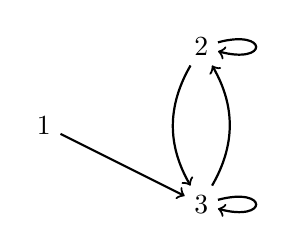
\begin{tikzpicture}
\node (atom1) at (0,1) {1};
\node (atom2) at (2,2) {2};
\node (atom3) at (2,0) {3};
\draw[->, thick] (atom1)--(atom3);
\draw[->, thick] (atom2) to[bend right] (atom3);
\draw[->, thick] (atom3) to[bend right] (atom2);
\draw[->, thick] (atom3) to[loop right, looseness=15] (atom3);
\draw[->, thick] (atom2) to[loop right, looseness=15] (atom2);
%\draw[->, thick] (atom4) to[loop right, looseness=15] (atom4);
\end{tikzpicture}

\end{multicols}



\begin{earg}
\item $\exists x Rxx$
\item $\forall x Rxx$
\item $\forall x \forall yRxy$
\item $\forall x\exists yRxy$
\item $\exists x \forall y Rxy$
%\item $\exists x \forall y Ryx$
\item $\exists x \forall y \enot Ryx$
\item $\forall y \exists x\enot Ryx$
\item $\forall x \forall y(Rxy \rightarrow Ryx)$
\item $\exists x\forall y(Rxy \rightarrow Ryx)$
\item $\forall x(\exists y Rxy \eif \exists y Ryx)$
%\item $\exists x \exists y (\enot x = y \eand Rxy \eand Ryx)$
%\item $\exists x \forall y(Rxy \eiff x = y)$
%\item $\exists x \forall y(Ryx \eiff x = y)$
%\item $\forall x \forall y \forall z ((Rxy \eand Ryz) \eif Rxz)$
%\item $\exists x \forall y \forall z ((Rxy \eand Ryz) \eif Rxz)$
%\item $\exists x \exists y(\enot x = y \eand Rxy \eand \forall z(Rzx \eiff y = z))$
\end{earg}

\problempart Determine the truth values of the sentences below on the provided interpretation (note that in the diagram, I am using an oval to indicate the extension of the 1-place predicate `$F$', and arrows for the extension of the 2-place predicate `$R$'):\\


\begin{minipage}{\textwidth}
\begin{multicols}{2}

	\begin{ekey}
		\item[\text{Domain}] 1, 2, 3
		\item[F] 1
		\item[R] \ntuple{1,1}, \ntuple{1,2}, \ntuple{1,3}, \ntuple{2,3}  \ntuple{3,2}, \ntuple{3,3}
		
	\end{ekey}

\columnbreak
	
\begin{tikzpicture}[>=stealth',thick]

\node (1) {1};
\node (2) [right=of 1] {2};
\node (3) [right=of 2] {3};



\draw (0,0) circle [x radius=0.6cm, y radius =1.2cm] node [left =0.5cm] {$F$};


\path (1) edge[->] (2);
\path (2) edge[->] (3);
\path (3) edge[->, bend right] (2);
\path (3) edge[->,loop above] (3);
\path (1) edge[->,bend right] (3);
\path (1) edge[->,loop above] (1);

\end{tikzpicture}
\end{multicols}
\end{minipage}




\begin{earg}

\item $\exists x(Fx \eand Rxx)$
\item $\exists x(\enot Fx \eand \enot Rxx)$
\item $\forall x(Rxx \rightarrow Fx)$
\item $\forall x(\exists yRxy \eif Fx)$
\item $\forall x\exists y Rxy$
\item $\forall x\exists yRxy \eif \exists xFx$
\item $\exists x(\forall y Rxy \eand \exists yRyx)$

\end{earg}




\section{Semantic Concepts}\label{s:FOLSemanticConcepts}

Defining truth in FOL was a bit tricky, due to the presence of quantifiers. But now that we know what determines the truth value of an FOL sentence in an interpretation, we can use that to define various other central logical notions.   As you can see, these definitions are basically the same as those from TFL, except that we here use the notion of truth in an \emph{interpretation} rather than truth on a \emph{valuation}.  In all the definitions below, the metavariables $\meta{\varphi}_1 \ldots \meta{\varphi}_n$ and $\meta{\psi}$ range over arbitrary \emph{sentences} of FOL:\footnote{Our logical concepts are in other words only defined for FOL sentences.  By contrast, the official explanation of truth in FOL, given in the Appendix, covers formulas in general, not just sentences.}

\factoidbox{
	$\meta{\varphi}_1, \ldots, \meta{\varphi}_n$ \define{logically entail}  $\meta{\psi}$, written $\meta{\varphi}_1, \ldots, \meta{\varphi}_n \vDash \meta{\psi}$,   iff no interpretation makes all of $\meta{\varphi}_1,  \ldots, \meta{\varphi}_n$ true but $\meta{\psi}$ false.\\

\meta{\varphi} is a \define{Logical Truth}, written $\vDash \meta{\varphi}$, iff it is true in every interpretation.\\

\meta{\varphi} is a \define{contradiction}  iff it is false in every interpretation.\\

\meta{\varphi} and \meta{\psi} are \define{logically equivalent}, written $\meta{\varphi} \lequiv \meta{\psi}$ iff they have the same truth value in every interpretation.\\

$\meta{\varphi}_1,\ldots, \meta{\varphi}_n$ are \define{jointly consistent} iff there is at least one interpretation which makes them all true.  They are \define{jointly inconsistent} iff there is no such interpretation.
}

As in TFL, perhaps the most important of these concepts is  entailment, since it is closely related to the notion of a valid argument.  We will say that an FOL argument:
$$\meta{\varphi}_1, \ldots, \meta{\varphi}_n \therefore \meta{\psi}$$
is \define{valid} just in case its premises $\meta{\varphi}_1, \ldots, \meta{\varphi}_n$ logically entail its conclusion \meta{\psi}.  Since entailment is defined in terms of the concept of truth-in-an-interpretation, we can use interpretations to investigate the validity of FOL arguments.

In particular, we can use interpretations to show that an argument is \emph{not} valid, or that the corresponding entailment \emph{fails}.  To show that a given argument is not valid, it suffices to construct a single interpretation that simultaneously makes all of the premises true but still makes the conclusion false.  Such an interpretation is again called a \emph{counterexample} to the validity of the argument, or a \define{countermodel}.


In the next two sections, we'll look at how to construct countermodels.  We'll first look at arguments that involve only one-place predicates, and then at ones that involve many-place predicates.  Of course, we can use interpretations to investigate the other logical concepts we've defined above too.  We'll return to that once we've looked at our central concept of entailment, or validity.

\section{Countermodels with One-Place Predicates}\label{s:CountermodelOnePl}

\paragraph{Example 1} Let's begin with one of the examples we looked at way back in \S\ref{s:Arguments}.

\begin{earg}
\item[]All rabbits are mammals
\item[] Bugs Bunny is a mammal.
\item[] $\therefore$ Bugs Bunny is a rabbit.
\end{earg}

\noindent As we noted at the time, this argument is intuitively not valid.  We are now in a position to demonstrate this formally.  First, we can offer the following FOL symbolization:
\begin{earg}
\item[] $\forall x(Rx \eif Mx)$
\item[] $Mb$
\item[] $\therefore$ $Rb$
\end{earg}
\noindent Next, we can construct an interpretation which makes the premises true and the conclusion false.  One such interpretation would be the following:
\begin{ekey}
	\item[\text{Domain}] all people
	\item[b] Lady Gaga
	\item[R] \blank \ is an opera singer
	\item[M] \blank\ is a vocalist
\end{ekey}
In this interpretation, `$\forall x(Rx \eif Mx)$' is  true, since every opera singer is a vocalist, and `$Mb$' is also true, since Lady Gaga is a vocalist.  But `$Rb$' is false, since she is not an opera singer, but a pop singer.  So the argument isn't valid.  However, using this kind of countermodel  has the drawback that it requires us to appeal to real-world knowledge.   After all, who knows, maybe, Lady Gaga secretly performs in operas too, in which case `$Rb$' is true in this interpretation, and it doesn't constitute a countermodel after all.

To avoid these kinds of issues, and to give some uniformity to our countermodels, we will again use interpretations with domains that contain just positive integers, and give \emph{direct} specifications of the extensions of predicates, by listing the objects they are true of.  Furthermore, since we may have to explain why universal sentences like `$\forall x(Rx \eif Mx)$' are true on our countermodels, and since the number of objects we have to consider to do this increases the larger the domain is, we will  try to construct countermodels  with the smallest possible domains.

Let's begin by seeing if we can construct a countermodel that has just one object in its domain, say the number 1.  First off, let's make sure our conclusion `$Rb$' is false.  To that end, we can let `$b$' refer to 1, and let the extension of the predicate `$R$' remain empty.  And to make the second premise, `$Mb$' true, we have to put 1 (the referent of `$b$') into the extension of `$M$'.  So we have an interpretation like this:

\begin{center}
\begin{minipage}{0.7\textwidth}
\begin{multicols}{2}
\begin{ekey}
	\item[\text{Domain}] 1
	\item[b] 1
	\item[R]
	\item[M] 1
\end{ekey}
\columnbreak
\begin{tabular}{c|c|c|c|}
\hline
 & &   R  & M  \\ \hline
b& 1   &   $-$  & $+$  \\ \hline
\end{tabular}
\end{multicols}\end{minipage}\end{center}
And luckily this also makes the first premise `$\forall x(Rx \eif Mx)$' true!  After all, $(Rx^1 \eif Mx^1)$ is true (since $Rx^1$ is false).  And since 1 is the only object in our domain, that suffices for `$\forall x(Rx \eif Mx)$'  to be true!  So our simple interpretation makes both premises true but the conclusion false, showing that the argument isn't valid.

\paragraph{Example 2} Let's look at a slightly more complex example:
$$\exists x(Fx \eif Gx) \therefore \exists xFx \eif \exists xGx$$
We will again begin with the smallest possible domain, containing just 1, and think about what's needed to make the conclusion, `$\exists xFx \eif \exists xGx$' false.  Since this is a conditional, we have to make its antecedent `$\exists x Fx$' true and its consequent `$\exists xGx$' false.  Using just the number 1, we can do that as follows:
\begin{center}\begin{tabular}{|c|c|c|}
\hline
&   F  & G  \\ \hline
1   &   $+$  & $-$  \\ \hline
\end{tabular}\end{center}
`$\exists xFx$' is now true, since $Fx^1$ is true.  But `$\exists xGx$' is false, because $Gx^1$ is false. The trouble is that this interpretation will also make our premise `$\exists x(Fx \eif Gx)$' false.  After all, $(Fx^1 \eif Gx^1)$ is false, and there's no other object in the domain we could assign to `$x$' to make `$(Fx \eif Gx)$' true.

So let's expand our domain by adding a second object:
\begin{center}\begin{tabular}{|c|c|c|}
\hline
&   F  & G  \\ \hline
1   &   $+$  & $-$  \\ \hline
2 &     ?    &  ?    \\ \hline
\end{tabular}\end{center}
We don't yet know whether our two predicates should be true or false of this new object, so I've left the cells next to it blank.  Let's begin with our conclusion `$\exists xFx \eif \exists xGx$' again: we want it to be false, so `$\exists xFx$' has to be true and `$\exists xGx$' has to be false.  Of course, `$\exists xFx$' remains true because $Fx^1$ is still true, so no change is needed here.  But to keep `$\exists xGx$' false, we need to make sure that our new object 2 is not in the extension of `$G$' either:
\begin{center}\begin{tabular}{|c|c|c|}
\hline
&   F  & G  \\ \hline
1   &   $+$  & $-$  \\ \hline
2 &     ?    &   $-$   \\ \hline
\end{tabular}\end{center}
Now, can we make the premise `$\exists x(Fx \eif Gx)$' true?  In fact we can, by making sure that `$F$' is not true of 2.  For in that case, $(Fx^2 \eif Gx^2)$ will be true, because the antecedent $Fx^2$ will be false.  And that suffices for the truth of `$\exists x(Fx \eif Gx)$'.  Our final countermodel, and the accompanying semantic demonstrations showing that our premise is true and our conclusion false, then look like this:

\begin{center}
\begin{minipage}{0.7\textwidth}
\begin{multicols}{2}
\begin{ekey}
	\item[\text{Domain}] 1, 2
	\item[F] 1
	\item[G]
\end{ekey}
\columnbreak
\begin{tabular}{|c|c|c|}
\hline
&   F  & G  \\ \hline
1   &   $+$  & $-$  \\ \hline
2 &     $-$    &   $-$   \\ \hline
\end{tabular}
\end{multicols}\end{minipage}\end{center}



\begin{ebullet}
\item $\exists x(Fx \eif Gx)$ is true because:
\begin{etriangle}
\item $(Fx^2 \eif Gx^2)$ is true (since $Fx^2$ is false)
\end{etriangle}
\end{ebullet}

\begin{ebullet}
\item $\exists xFx \eif \exists x Gx$ is false because:
\begin{etriangle}
\item $\exists xFx$ is true
\begin{etriangle}
\item since $Fx^1$ is true
\end{etriangle}
\item but $\exists xGx$ is false.  This is because
\begin{etriangle}
\item $Gx^1$ is false, and
\item $Gx^2$ is also false
\end{etriangle}
\end{etriangle}
\end{ebullet}


We only needed a single object in the domain of our first countermodel, but our second countermodel ended up requiring two objects to simultaneously make the premises true and the conclusion false.  Other examples might require you to use three objects, or even four, or more.  Is there any upper bound on the number of objects that might be needed to produce a countermodel?

It turns out that for arguments that only involve one-place predicates, the answer is `yes'.  The logician Leopold L\"owenheim showed that if an FOL argument contains just $n$ one-place predicates, then if the argument is invalid, a countermodel with a domain of at most $2^n$ objects exists.  So for something like Example 2, which involves two one-place predicates, we can be sure that we won't need more than four objects.  As we'll see, there is no such upper bound for arguments with many-place predicates.


Before we turn to many-place predicates, though, one more general observation is in order.  Consider the following English argument:
\begin{earg}
	\item[] All foxes are mortal.
	\item[$\therefore$] Every vixen is mortal.
\end{earg}
This argument is valid in the sense that it's impossible for its premise to be true but its conclusion to be false: a vixen is just a female fox, so any possible world where every fox is mortal has to be one where every vixen is mortal.  But if we symbolize it, the resulting FOL argument is \emph{not} valid:
\begin{earg}
	\item[] $\forall x(Fx \eif Mx)$
	\item[$\therefore$] $\forall x(Vx \eif Mx)$
\end{earg}
It's easy to construct an interpretation that makes the premise true and the conclusion false (just put an object in the extension of $V$ but not $M$ or $F$).

So from the fact that the symbolization of an English argument in FOL is not valid, we can't straightaway conclude that the original English argument is not valid.   What we can conclude is just that the original English argument is not \emph{formally} valid, or more specifically, that it isn't valid in virtue of the kind of logical form captured in its FOL symbolization.  But it might still be valid for other reasons --- in this case, because of the connection between the meanings of `fox' and `vixen'.  As we discussed in \S\ref{s:FormalValidity}, logic doesn't aim to capture the validity of arguments like this; it only cares about formally valid arguments.\footnote{Of course we can make the above argument formally valid by adding a second premise: `Every vixen is a fox', which we'd symbolize as `$\forall x(Vx \eif Fx)$'.  But this is now a \emph{different}  $FOL$ argument, one with two premises.}

\practiceproblems
\problempart Construct countermodels to demonstrate the following:

\begin{earg}
\item $\forall xFx \eiff \forall x Gx \nvDash \forall x(Fx \eiff Gx)$ % Needs 1
\item $\forall x ((Fx \eand Gx) \eif Hx) \nvDash \forall x(Fx \eor Gx) \eor \forall x(Fx \eor Hx)$ %Needs 1
\item $\forall xFx \eif \exists xGx \nvDash \exists x Fx \eif \exists x Gx$ % Needs 2
\item $(\forall x Fx \eand \forall x Gx) \eif \forall x Hx \nvDash \forall x((Fx \eand Gx) \eif Hx)$ % Needs 2
\item $\exists x\forall y(Fx \eif Gy) \nvDash \exists y\forall x(Fx \eif Gy)$
\item $\forall x \exists y(Fy \eif Gx) \nvDash \forall x(\exists yFy \eif Gx)$ % Needs 2
\item $\forall x(\exists yFy \eif Gx) \nvDash \forall x \exists y(Fy \eif Gx)$
\end{earg}



\section{Countermodels with Many-Place Predicates}

Let's next look at how to construct countermodels for arguments with many-place predicates.  First, though, there's some new terminology that will come in handy.  Two-place predicates like `loves', `respects', `admires' etc. express \define{relations} between objects (the loving relation, the respecting relation, and so on).  And there are some important characteristics that relations like this can have:

\factoidbox{
A relation $R$ is \define{serial} iff $\forall x \exists y Rxy$

A relation $R$ is \define{reflexive} iff $\forall xRxx$

A relation $R$ is \define{symmetric} iff $\forall x \forall y(Rxy \eif Ryx)$

A relation $R$ is \define{transitive} iff $\forall x \forall y \forall z((Rxy \eand Ryz) \eif Rxz)$
}
One thing we can do, then, is to show that a relation's having certain of these characteristics does, or does not, imply its having some other characteristic.  For example, being reflexive implies being serial. After all: if every object bears $R$ to itself, then every object bears $R$ to \emph{at least} one thing, namely itself!  You could do a natural deduction proof to show that $\forall x Rxx \vdash \forall x \exists y Rxy$.  However, the implication does not hold in the other direction, i.e. being serial does \emph{not} imply being reflexive.  Showing this will be our first example.

\paragraph{Example 1} $\forall x \exists y Rxy \nvDash \forall xRxx$

You can perhaps already think of a countermodel that would make `$\forall x \exists y Rxy$' true but `$ \forall xRxx$' false, but again, we're going to try to find the smallest countermodel to do the job.  Let's start with a domain that just contains the number 1.  For `$\forall x \exists y Rxy$' to be true, every object in the domain has to bear the relation $R$ to at least one object.  So since we only have one object, that means 1 has to bear $R$ to itself:
\begin{center}
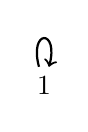
\begin{tikzpicture}
\node (atom1) {1};
\draw[->, thick] (atom1) to[loop above] (atom1);
\end{tikzpicture}
\end{center}
However, this now also makes `$\forall xRxx$' true, whereas our goal is to make this false.

So let's expand our domain to include two objects, 1 and 2.  In order for `$\forall xRxx$' to be false, at least one of these objects must not bear $R$ to itself, i.e. must not have an arrow looping back to itself.  And for `$\forall x\exists yRxy$' to be true, every object has to bear $R$ to something, i.e. must have at least one outgoing arrow.  One easy way to achieve both is to expand our earlier model to look like this:

\begin{center}
\begin{minipage}{0.8\textwidth}
\begin{multicols}{2}
\begin{ekey}
	\item[\text{Domain}] 1, 2
	\item[R] \ntuple{1,1}, \ntuple{2,1}
\end{ekey}
\columnbreak
\begin{tikzpicture}
\node (atom1) {1};
\node (atom2) [right=of atom1] {2};

\draw[thick,->] (atom2) to[->] (atom1);
\draw[thick,->] (atom1) to[->, loop above] (atom1);
\end{tikzpicture}
\end{multicols}\end{minipage}\end{center}
The accompanying semantic demonstration runs like this:

\begin{ebullet}
\item $\forall x \exists y Rxy$ is true because:
\begin{etriangle}
\item $\exists yRx^1y$ is true
\begin{etriangle}
\item since $Rx^1y^1$ is true
\end{etriangle}
\item and $\exists yRx^2y$ is also true
\begin{etriangle}
\item since $Rx^2y^1$
\end{etriangle}
\end{etriangle}
\end{ebullet}

\begin{ebullet}
\item $\forall xRxx$ is false because:
\begin{etriangle}
\item $Rx^2x^2$ is false
\end{etriangle}
\end{ebullet}

There are of course many other countermodels that would do the job just as well.  But what we have in any case discovered is that \emph{at least two} objects are necessary to show that the entailment from seriality to reflexivity fails.

\paragraph{Example 2} Next, let's show the following:
$$\forall x Lxx, \forall x\forall y(Lxy \eif Lyx) \nvDash \exists x\forall yLxy$$
That is: a relation $L$'s being both reflexive and symmetric does not imply that that there is some object $x$ that bears $L$ to everything (there's no official name for this latter characteristic).  If we begin with a domain containing just 1, then to make `$\forall xLxx$' true, we would have to do the following:
\begin{center}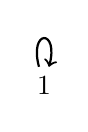
\begin{tikzpicture}
\node (atom1) {1};
\draw[->, thick] (atom1) to[loop above] (atom1);
\end{tikzpicture}\end{center}
However, since we want to make `$\exists x\forall yLxy$' \emph{false}, we need to make sure that for every $x$, there is at least one object it \emph{doesn't} bear $L$ to, i.e. we want the following to hold: $\forall x \exists y \enot Lxy$.  And the trouble is that as things stand, every object \emph{does} bear $L$ to something.

So let's try it with two objects.  Again, to make `$\forall xLxx$' true, they both need to bear $L$ to themselves:
\begin{center}\begin{tikzpicture}
\node (atom1) {1};
\node (atom2) [right=of atom1] {2};
\draw[->, thick] (atom1) to[loop above] (atom1);
\draw[->, thick] (atom2) to[loop above] (atom2);
\end{tikzpicture}\end{center}
Notice that at this point, `$\forall x \exists y \enot Lxy$' holds.  For every object we can find at least one thing it doesn't bear $L$ to: 1 doesn't bear $L$ to 2, and 2 doesn't bear $L$ to 1.  We still have to make sure that symmetry holds, i.e. that `$\forall x\forall y(Lxy \eif Lyx)$' is true.  But if you think about it, symmetry does hold in our diagram: everything that 1 bears $L$ to --- which is just itself --- also bears $L$ back to 1.  And similarly, everything that 2 bears $L$ to --- which is just itself --- also bears $L$ back to 2.  So we're done!  Our countermodel and accompanying semantic demonstration (which gets pretty involved in the case of symmetry!) looks like this:
\begin{center}
\begin{minipage}{0.8\textwidth}
\begin{multicols}{2}
\begin{ekey}
	\item[\text{Domain}] 1, 2
	\item[R] \ntuple{1,1}, \ntuple{2,2}
\end{ekey}
\columnbreak
\begin{tikzpicture}
\node (atom1) {1};
\node (atom2) [right=of atom1] {2};
\draw[->, thick] (atom1) to[loop above] (atom1);
\draw[->, thick] (atom2) to[loop above] (atom2);
\end{tikzpicture}
\end{multicols}\end{minipage}\end{center}

\begin{ebullet}
\item $\forall xLxx$ is true because:
\begin{etriangle}
\item $Lx^1x^1$ is true, and
\item $Lx^2x^2$ is also true
\end{etriangle}
\end{ebullet}

\begin{ebullet}
\item $\forall x\forall y(Lxy \eif Lyx)$ is true because:
\begin{etriangle}
\item $\forall y(Lx^1y \eif Lyx^1)$ is true, since:
\begin{itemize}
\item $(Lx^1y^1 \eif Ly^1x^1)$ is true (because $Lx^1y^1$ and $Ly^1x^1$ are both true), and
\item $(Lx^1y^2 \eif Ly^2x^1)$ is also true (because $Lx^1y^2$ is false)
\end{itemize}

\item and $\forall y(Lx^2y \eif Lyx^2)$ is true, since:
\begin{etriangle}
\item $(Lx^2y^1 \eif Ly^1x^2)$ is true (because $Lx^2y^1$ is false), and
\item $(Lx^2y^2 \eif Ly^2x^2)$ is also true (because $Lx^2y^2$ and $Ly^2x^2$ are both true)
\end{etriangle}
\end{etriangle}
\end{ebullet}

\begin{ebullet}
\item $\exists x\forall yLxy$ is false because:
\begin{etriangle}
\item $\forall y Lx^1y$ is false, since:
\begin{itemize}
\item $Lx^1y^2$ is false
\end{itemize}
\item and $\forall y Lx^2y$ is also false, since
\begin{etriangle}
\item $Lx^2y^1$ is false
\end{etriangle}
\end{etriangle}
\end{ebullet}

Again, the countermodel we arrived at is not the only one possible.  The following would work too, for example, and might be more intuitive:
\begin{center}
\begin{tikzpicture}
\node (atom1) {1};
\node (atom2) [right=of atom1] {2};
\node (atom3) [right=of atom2] {3};
\draw[->, thick] (atom1) to[loop above] (atom1);
\draw[->, thick] (atom2) to[loop above] (atom2);
\draw[->, thick] (atom3) to[loop above] (atom3);
\draw[->, thick] (atom1) to[bend right] (atom2);
\draw[->, thick] (atom2) to[bend right] (atom1);
\draw[->, thick] (atom2) to[bend right] (atom3);
\draw[->, thick] (atom3) to[bend right] (atom2);
\end{tikzpicture}
\end{center}
But with three objects in the domain, giving a semantic demonstration would require more work.  To show that `$\forall x\forall y(Lxy \eif Lyx)$' holds, for example, we'd have to show that `$\forall y(Lxy \eif Lyx)$' is true no matter which of our three objects we assign to `$x$'; and then relative to each choice for `$x$', we'd have to show that `$(Lxy \eif Lyx)$' is true no matter what we assign to `$y$'.  So we'd have to consider nine different assignments of objects to `$x$' and `$y$' in total, whereas the demonstration above only required us to look at four assignments.

\practiceproblems
\problempart Construct countermodels to demonstrate the following:

\begin{earg}

\item $\forall x \exists y Lxy \nvDash \exists x \forall y Lxy$ % Needs 2
\item $\forall x \exists yLyx \nvDash \forall x \exists yLxy$
\item $\exists x(Fx \eand \forall y Rxy) \nvDash \forall x(Fx \eif \exists yRxy)$ % Needs 2
\item $\exists x(\exists yAxy \eand \enot \exists y Ayx) \nvDash \exists x \forall y(Axy \eif Ayx)$
\item $\forall x(\forall yRxy \eif \exists z \forall wRwz) \nvDash \forall x \exists y \forall z(Rxy \eiff Rzy)$
\end{earg}


\section{Validity and Decidability}

Let's investigate one more argument involving a two-place predicate:
$$\forall x\exists yRxy, \forall x \forall y \forall z((Rxy \eand Ryz) \eif Rxz) \therefore \exists xRxx$$
For this to be valid, the seriality and transitivity of $R$ would together have to imply that some object bears $R$ to itself (again, there's no official name for this latter characteristic).  Let's see if we can construct a countermodel.

To make the conclusion `$\exists xRxx$' false, we have to make sure that \emph{no} object in our interpretation bears $R$ to itself, i.e. there can be no arrows that loop from an object onto itself.  And as we already noticed at the hand of Example 1 in the previous section, for seriality to hold in a domain of just one object, that object would have to bear the relation to itself.  So we cannot make seriality true and `$\exists xRxx$' false with just one object.

So let's move to a domain with two objects.  We can make seriality hold while avoiding any self-looping arrows like this:
\begin{center}
\begin{tikzpicture}
\node (atom1) {1};
\node (atom2) [right=of atom1] {2};

\draw[thick,->] (atom2) to[bend right] (atom1);
\draw[thick,->] (atom1) to[bend right] (atom2);
\end{tikzpicture}
\end{center}
But now consider how to make transitivity, i.e. `$\forall x \forall y \forall z((Rxy \eand Ryz) \eif Rxz)$', hold.  For this to be true, the conditional `$(Rxy \eand Ryz) \eif Rxz$' has to be true no matter which objects we assign to each of the variables `$x$', `$y$', and `$z$'. So suppose we assign  2 to `$y$', and 1 to both `$x$' and `$z$': $(Rx^1y^2 \eand Ry^2z^1) \eif Rx^1z^1$.  Both $Rx^1y^2$ and $Ry^2z^1$ are true, so for the latter conditional to be true, the consequent $Rx^1z^1$ has to be true.  But this would now require a self-looping arrow from $1$ back to $1$!  So we can't get what we want with just two objects.

Let's try three objects.  What we've just seen is that we can't have any symmetric arrows, since that would introduce a self-looping arrow by transitivity.  With three objects, we can secure seriality (making sure every object has an arrow going to some object) while avoiding both symmetric and self-looping arrows like this:
\begin{center}
\begin{tikzpicture}[>=stealth',thick]

\node (1) {1};
\node (2) [right=of 1] {2};
\node (3) [right=of 2] {3};

\draw[->,thick] (1) to (2);
\draw[->,thick] (2) to (3);
\draw[->,thick] (3) to[bend left] (1);

\end{tikzpicture}
\end{center}
But again, transitivity causes a problem.  Let's assign 2 to `$x$', 3 to `$y$', and 1 to `$z$', giving us: $(Rx^2y^3 \eand Ry^3z^1) \eif Rx^2z^1$.  Since both $Rx^2y^3$ and $Ry^3z^1$ are true, for the conditional to be true, the consequent $Rx^2z^1$ has to be true.   That would mean adding an arrow going from 2 to 1.  But since we already have an arrow going from 1 to 2,  that would reintroduce a double-headed arrow!

What this shows is that we can't have any arrows that ``go backward'' in our interpretation, to an earlier number.  We could add a fourth object so that 3's arrow can move forward:
\begin{center}
\begin{tikzpicture}[>=stealth',thick]

\node (1) {1};
\node (2) [right=of 1] {2};
\node (3) [right=of 2] {3};
\node (4) [right=of 3] {4};
\node (5) [below=1.5em of 4] {?};

\draw[->,thick] (1) to (2);
\draw[->,thick] (2) to (3);
\draw[->,thick] (3) to (4);
\draw[->,thick] (4) to[bend left] (5);

\end{tikzpicture}
\end{center}
But 4 \emph{also} has to have an arrow going to some object (for seriality).  And that arrow can't go backward to 1, 2, or 3, and can't go from 4 to itself, so what's to be done? Does this mean it's impossible to construct a countermodel, and that our argument is therefore valid?

No, it does not: the argument is invalid, and a countermodel exists, but it requires \emph{infinitely many objects} in its domain.  The following is a countermodel, for example:
\begin{ekey}
	\item[\text{Domain}] all positive integers
	\item[R] \blank \ is less than \blank \ (or: all pairs of integers \ntuple{m,n} where $m < n$)
\end{ekey}
We can't specify this interpreation ``directly'' by listing all the objects in the domain and all the pairs in the extension of `$R$', since there are too many of them.  But we can specify the extension of `$R$' indirectly, via the English predicate. This interpretation does what we want:
\begin{ebullet}
\item `$\forall x\exists yRxy$' is true, since for every positive integer $x$ we can find a $y$ such that $x<y$
\item `$\forall x \forall y \forall z((Rxy \eand Ryz) \eif Rxz)$' is true, since if $x < y$ and $y < z$, it follows that $x < z$.
\item `$\exists xRxx$' is false, since there exist no integer $x$ such that $x < x$.
\end{ebullet}

What we've seen, then, is that showing an FOL argument to be invalid may require an interpretation with infinitely many objects.  As mentioned in \S\ref{s:CountermodelOnePl}, this is not the case for FOL arguments that contain only \emph{one-place} predicates.  If such an argument is invalid, then there exists a countermodel with a domain of at most $2^n$ objects (where $n$ is the number of one-place predicates the argument contains).  Since there are finitely many interpretations for $n$ predicates using at most $2^n$ objects, this means that a computer could in principle crunch through all of those interpretations and determine if the argument is valid: if it finds a countermodel among them, the argument is invalid, if it doesn't, the argument is valid.

The same holds for TFL.  Any TFL argument can be tested for validity by constructing its joint truth table and checking wether any line (i.e. valuation) makes all the premises true and the conclusion false.  So a computer can be programmed to mechanically test any TFL argument for validity.

What we've seen is that this does not hold for FOL arguments that contain two-place predicates.  Here there is no finite number of interpretations we could program a computer to check such that, if it fails to find a countermodel among them, the argument is guaranteed to be valid.  And in fact, as the logicians Alan Turing and Alonzo Church independently proved in 1936, there exists \emph{no} mechanical test for validity in FOL. Validity in FOL is therefore said to be \define{undecidable}, in contrast to TFL, where validity is \define{decidable} via truth-tables.


Demonstrating FOL arguments to be valid therefore invariably requires some ingenuity and insight --- it's not the kind of thing a computer can do. This is why we use natural deduction proofs to demonstrate validity in FOL: if methods that require ingenuity are going to be required anyhow, we might as well use the method of natural deduction.\footnote{Of course, by using natural deductions to demonstrate validity, we are relying on the fact that our proof system is sound, i.e. only lets us prove valid arguments.  See the introduction to Chapter \ref{ch:NDFOL} on this concept.}
To be sure, one \emph{can} also give semantic proofs to demonstrate the validity of FOL arguments.  For example to show that the following entailment holds:
$$\exists x(Fx \eand Gx) \vDash \exists x Fx \eand \exists xGx$$
we could give the following semantic proof in English:
\begin{itemize}
\item[] \emph{Semantic Proof:} consider some arbitrary interpretation \meta{I}, and suppose $\exists x(Fx \eand Gx)$ is true in \meta{I}.  This means there is some object in the domain of \meta{I}, let's call it $a$, such that $(Fx^a \eand Gx^a)$ is true in \meta{I}.  But then since $Fx^a$ is true in \meta{I}, this means $\exists xFx$ is true in \meta{I}.  And similarly, since $Gx^a$ is true in \meta{I}, it follows that $\exists xGx$ must be true in \meta{I}.  Therefore $\exists x Fx \eand \exists xGx$ is true in \meta{I}.  Since \meta{I} was an arbitrary interpretation, we can conclude that \emph{every} interpretation that makes $\exists x(Fx \eand Gx)$ true must also make $\exists x Fx \eand \exists xGx$ true, meaning that the entailment above holds.
\end{itemize}
However, we can also give a natural deduction proof, which goes through a very similar line of reasoning:
\begin{proof}
	\hypo{1}{\exists x (Fx \eand Gx)} \by{Premise}{}
	\open
		\hypo{2}{Fa \eand Ga} \by{Assumption (flag a)}{}
		\have{3}{Fa}\ae{2}
		\have{4}{\exists xFx} \Ei{3}
		\have{5}{Ga}\ae{2}
		\have{6}{\exists xFx} \Ei{5}
		\have{7}{\exists xFx \eand \exists xGx} \ai{4,6}
	\close
	\have{7}{\exists xFx \eand \exists xGx} \Ee{1,2-7}
\end{proof}
Natural deduction proofs do not, however, allow use to demonstrate that arguments are \emph{invalid}.  To do this, we have to rely on the method of constructing countermodels.  And that's what we have been doing in the last several sections.


\section{Working with Other Semantic Concepts}


So far, we've just been focusing on validity, or entailment. But we can use interpretations, as well as natural deduction proofs, in connection with other semantic concepts too.

Take the concept of logical truth first.  To show that some FOL sentence \meta{\varphi} is \emph{not} a logical truth, it suffices to construct an interpretation that makes it false.  And to show that it \emph{is} a logical truth, we can give a natural deduction that proves \meta{\varphi} as a theorem.  This gives us a way to approach contradictions as well: since \meta{\varphi} is a contradiction iff $\enot\meta{\varphi}$ is a logical truth, we can show that \meta{\varphi} is a contradiction by proving $\enot\meta{\varphi}$ as a theorem.  And to show that \meta{\varphi} is \emph{not} a contradiction, it suffices to construct an interpretation in which it is true.


Next consider logical equivalence.  To show that \meta{\varphi} and \meta{\psi} are \emph{not} logically equivalent, all we need to do is construct an interpretation on which one of them is true and the other is false.  And to show that \meta{\varphi} and \meta{\psi} \emph{are} equivalent, we can give a natural deduction that proves $\meta{\varphi} \eiff \meta{\psi}$ as a theorem, since \meta{\varphi} and \meta{\psi} are equivalent just in case $\meta{\varphi} \eiff \meta{\psi}$ is a logical truth.


Lastly, take the concept of consistency.  To show that some sentences are jointly consistent, it suffices to give an interpretation on which they are all true.  As for inconsistency, notice that it connects to entailment in the following way:
\factoidbox{$$\text{If } \meta{\varphi}_1, \ldots, \meta{\varphi}_n \entails \bot \text{, then } \meta{\varphi}_1, \ldots, \meta{\varphi}_n \text{ are jointly inconsistent} $$
}
For suppose  $\meta{\varphi}_1, \ldots, \meta{\varphi}_n \entails \bot$.  This means there's no interpretation that makes all of $\meta{\varphi}_1, \ldots, \meta{\varphi}_n $ true but $\bot$ false.  However, since every interpretation makes $\bot$ false, this just means that there's no interpretation that makes all of $\meta{\varphi}_1, \ldots, \meta{\varphi}_n $ true.  That is, $\meta{\varphi}_1, \ldots, \meta{\varphi}_n $ are inconsistent.    So if we want to show that $\meta{\varphi}_1, \ldots, \meta{\varphi}_n $ are inconsistent, we can do that by giving a natural deduction proof showing that $\meta{\varphi}_1, \ldots \meta{\varphi}_n \proves \bot $.

The following table summarizes what is needed to demonstrate that a given concept does or does not apply:
\begin{center}
\begin{tabular}{l l l}
%\cline{2-3}
 & \textbf{Yes} & \textbf{No}\\
 \hline
%\cline{2-3}
logical truth? & give a proof & give an interpretation\\
contradiction? &  give a proof  & give an interpretation\\
equivalent? & give a proof & give an interpretationl\\
consistent? & give an interpretation & give a proof\\
valid? & give a proof & give an interpretation\\
entailment? & give a proof & give an interpretation\\
\end{tabular}
\end{center}


\practiceproblems

%\problempart
%Give counermodels to show the following:
%
%\begin{earg}
%\item $\forall x(Ax \eif Bx) \nvDash \exists x Bx$
%\item $\forall x(Rx \eif Dx), \forall x(Rx \eif Fx) \nvDash \exists x(Dx \eand Fx)$
%\item $\exists x(Px\eif Qx) \nvDash \exists x Px$
%\item $Na \eand Nb \eand Na \nvDash \forall x Nx$
%\item $\exists x(Ex \eand Fx), \exists x Fx \eif \exists x Gx \nvDash \exists x(Ex \eand Gx)$
%\item $Rab, \exists x Rxa \nvDash Rba$
%\item $\forall x Oxa, \forall x Oax \nvDash \forall x Oxx$
%\item $\forall x \exists yLxy \nvDash \exists x \forall yLxy$
%\item $\exists x(Jx \eand Kx), \exists x \enot Kx, \exists x \enot Jx \nvDash \exists x(\enot Jx \eand \enot Kx)$
%\item $Lab \eif \forall x Lxb, \exists x Lxb \nvDash Lbb$
%\item $\forall x(Dx \eif \exists y Tyx) \nvDash \exists y \exists z\  y \neq z$
%\item $\forall x (Fx \eor \enot Gx) \nvDash (\forall x Fx \eor \enot \exists x Gx)$
%\item $\forall x\exists y(Rxy \eif Rxx) \nvDash \forall x(\exists yRxy \eif Rxx)$
%\item $\forall xFx \eiff \forall yGy \nvDash \forall x(Fx \eiff AyGy)$
%\item $\forall x \exists yRxy , \exists x\forall yRxy \nvDash \forall x \forall y Rxy$
%\item $\nvDash \exists x \forall y((Rxy \land \sim Ryx) \rightarrow (Rxx \leftrightarrow Ryy))$
%\end{earg}

%\problempart
%\label{pr.Contingent}
%Show that each of the following is neither a logical truth nor a contradiction (by constructing an interpretation for each that makes it true, and one that makes it false):
%\begin{earg}
%\item  $Da \eand Db$
%\item  $\exists x Txh$
%\item  $Pa \eand \enot\forall x Px$
%\item $\forall z Jz \eiff \exists y Jy$
%\item $\forall x (Rxa \eor \exists yLxy)$
%\item $\exists x (Gx \eif \forall y My)$
%%\item $\exists x (x = h \eand x = i)$
%\item $\exists x \forall y((Rxy \eand \enot Ryx) \eif (Rxx \eiff Ryy))$
%\end{earg}

\problempart
\label{pr.NotEquiv}
Show that the following pairs of sentences are not logically equivalent (by constructing an interpretation for each pair that makes one true but the other false):
\begin{earg}
\item $\exists x Jx$, $\exists x \lnot Jx$
\item $\exists x Jx \land \exists x Hx, \exists x(Jx \land Hx)$
\item $\forall x Rxx$, $\exists x Rxx$
\item $\exists x Px \eif \exists yQy$, $\exists x (Px \eif \exists yQy)$
\item $\forall x(Px \eif \enot Qx)$, $\exists x(Px \eand \enot Qx)$
\item $\exists x(Px \eand Qx)$, $\exists x(Px \eif Qx)$
\item $\forall x(Px\eif Qx)$, $\forall x(Px \eand Qx)$
\item $\forall x\exists y Rxy$, $\exists x\forall y Rxy$
\item $\forall x\exists y Rxy$, $\forall x\exists y Ryx$
\end{earg}



\problempart
Show that the following sentences are jointly consistent (i.e. there's an interpretation that makes them all true):
\begin{earg}
%\item $Ma, \enot Na, Pa, \enot Qa$
%\item $La, Lab, \enot Lbe, \enot Lbb$
%\item $\enot (Ma \eand \exists x Ax), Ma \eor Fa, \forall x(Fx \eif Ax)$
%\item $Ma \eor Mb, Ma \eif \forall x \enot Mx$
\item $\forall y Gy, \forall x (Gx \eif Hx), \exists y \enot Iy$
\item $\exists x(Bx \eor Ax), \forall x \enot Cx, \forall x\bigl[(Ax \eand Bx) \eif Cx\bigr]$
\item $\exists x Xx, \exists x Yx, \forall x(Xx \eiff \enot Yx)$
\item $\forall x(Px \eor Qx), \exists x\enot(Qx \eand Px)$
\item $\exists z(Nz \eand Ozz), \forall x\forall y(Oxy \eif Oyx)$
\item $\enot \exists x \forall y Rxy, \forall x \exists y Rxy$
%\item $\enot Raa$, $\forall x (x=a \eor Rxa)$
%\item $\forall x\forall y\forall z(x=y \eor y=z \eor x=z)$, $\exists x\exists y\ \enot x= y$
%\item $\exists x\exists y(Zx \eand Zy \eand x=y)$, $\enot Zd$, $d=e$
\end{earg}

%\problempart
%\label{pr.FOLequivornot}
%For each of the following pairs of sentences, if they are provably equivalent, give proofs to show this, and if they are not, construct countermodel to show they are not equivalent:
%\begin{earg}
%\item $\forall x Px \eif \exists yQy, \forall x (Px \eif \exists yQy)$
%\item $\forall x\forall y \forall z Bxyz, \forall x Bxxx$
%\item $\forall x\forall y Dxy, \forall y\forall x Dxy$
%\item $\exists x\forall y Dxy, \forall y\exists x Dxy$
%\item $\forall x (Rba \eiff Rxa), Rba \eiff \forall x Rxa$
%\end{earg}

%\problempart
%\label{pr.FOLvalidornot}
%For each of the following arguments: if it is valid in FOL, give a proof. If it is invalid, construct an interpretation to show that it is invalid.
%\begin{earg}
%\item $\exists y\forall x Rxy \therefore \forall x\exists y Rxy$
%\item $\exists x(Px \eand \enot Qx) \therefore \forall x(Px \eif \enot Qx)$
%\item $\forall x(Sx \eif Ta), Sb \therefore Ta$
%\item $\forall x(Ax\eif Bx), \forall x(Bx \eif Cx) \therefore \forall x(Ax \eif Cx)$
%\item $\exists x(Dx \eor Ex), \forall x(Dx \eif Fx) \therefore \exists x(Dx \eand Fx)$
%\item $\forall x\forall y(Rxy \eor Ryx) \therefore Raa$
%\item $\exists x\exists y(Rxy \eor Ryx) \therefore Raa$
%\item $\forall x Px \eif \forall x Qx, \exists x \enot Px \therefore \exists x \enot Qx$
%\end{earg}


\section{Semantics for Identity}

As mentioned in  \S\ref{s:identity}, FOL is standardly supplemented with a primitive logical symbol $=$ for \emph{identity}. In \S\ref{s:identityrules} we looked at the deduction rules that govern identity, with which we were then able to prove various logical truths involving identity, like that everything is identical to itself, $\forall x  \ x=x$.

Similarly, we now need to say something about the semantics of identity, specifically how to determine the truth values of identity statements in an interpretation.  In this case, the semantics is very simple:%\footnote{This clause assumes that variables can refer to objects, but technically variables only refer \emph{relative to} an assignment of values.  Again, see the Appendix in \S\ref{s:semanticsappendix} below for the official semantics, that makes the role of variable assignments explicit.}
\factoidbox{
		For any names $\meta{a}$ and $\meta{b}$, $\meta{a} = \meta{b}$ is true in a given interpretation \textbf{iff}  \meta{a} and \meta{b} refer to very same object in that interpretation.
}
So if, for example, our interpretation specifies that the name `$m$' refers to 1, that `$n$' refers to 2, and that `$o$' also refers to 2, then `$m = n$' would be false (since 1 and 2 aren't identical) whereas `$n = o$' would be true (since 2 is identical to 2).  And of course, things like `$m = m$' or `$n = n$' will always be true, on any interpretation, since \emph{whatever} `$n$' (or `$m$') refers to, it will be identical to itself.


This clause only covers identity statements involving names.  For identity statements involving variables, we again have to bring in variable assignments.  E.g. `$x=y$' comes out true if the variables `$x$' and `$y$' are both assigned the value 1, say, but it would come out false if `$x$' were assigned the value 1 and `$y$' the value $2$.  On the other hand, `$x=x$' comes out true no matter what value is assigned to `$x$'.  See the Appendix in \S\ref{s:semanticsappendix} below for the official semantics that makes the role of variable assignments explicit.


We can also consider quantified sentences involving identity.  In \S\ref{s:identity} we saw how to symbolize numerical claims using identity.  The claim that exactly one object exists can, for example, be symbolized as `$\exists x \forall y \ x = y$', and the claim that exactly two objects exist can be symbolized as `$\exists x \exists y( x \neq y \eand \forall z(z = x \eor z = y))$'.\footnote{Again, $x \neq y$ is jus shorthand for $\enot (x = y)$}   Using our semantics, we can now show that `$\exists x \forall y \ x = y$' is indeed false if the domain contains more than one object:

\begin{center}

\begin{ekey}
	\item[\text{Domain}] 1, 2
\end{ekey}
\end{center}

\begin{ebullet}
\item[] $\exists x \forall y \ x = y$ is false because:
\begin{etriangle}
\item $\forall y \ x^1 = y$ is false
\begin{etriangle}
\item since $x^1 = y^2$ is false.
\end{etriangle}
\item and $\forall y \ x^2 = y$ is also false
\begin{etriangle}
\item since $x^2 = y^1$ is false.
\end{etriangle}
\end{etriangle}
\end{ebullet}
Similarly, we could show that `$\exists x \exists y( x \neq y \eand \forall z(z = x \eor z = y))$', that is, the claim that exactly two objects exist, is false on a domain that contains 1, 2, and 3. (Though for this, the complete semantic demonstration would be quite long, since there are three possible values to consider for `$x$', and then three possible values for `$y$' in each case!)


\practiceproblems

\problempart Consider again the following interpretation:

\begin{multicols}{2}
	\begin{ekey}
		\item[\text{Domain}] 1, 2, 3
		\item[R] \ntuple{1,3}, \ntuple{2,2}, \ntuple{2,3}, \ntuple{3, 2} \ntuple{3,3}
	\end{ekey}
\columnbreak

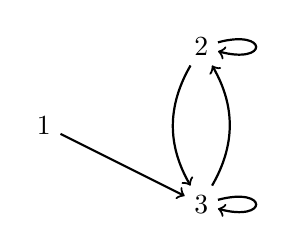
\begin{tikzpicture}
\node (atom1) at (0,1) {1};
\node (atom2) at (2,2) {2};
\node (atom3) at (2,0) {3};
\draw[->, thick] (atom1)--(atom3);
\draw[->, thick] (atom2) to[bend right] (atom3);
\draw[->, thick] (atom3) to[bend right] (atom2);
\draw[->, thick] (atom3) to[loop right, looseness=15] (atom3);
\draw[->, thick] (atom2) to[loop right, looseness=15] (atom2);
%\draw[->, thick] (atom4) to[loop right, looseness=15] (atom4);
\end{tikzpicture}

\end{multicols}


\noindent Determine whether each of the following sentences is true or false in this interpretation, and give a semantic demonstration to justify your answer.
\begin{earg}
\item $\forall x (\exists y \ x \neq y \eand \exists y \ x = y)$
\item $\forall x \exists y ( x \neq y \eand \ x = y)$
\item $\exists x \forall y \ x = y$
\item $\exists x \exists y (x \neq y \eand  (Rxy \eand Ryx))$
\item $\exists x \forall y(Rxy \eiff x = y)$
\item $\exists x \forall y(Ryx \eiff x = y)$
\item $\exists x \exists y((x \neq y \eand Rxy) \eand \forall z(Rzx \eiff y = z))$
\end{earg}


\problempart
\label{pr.Contingent}
Show that each of the following is neither a logical truth nor a contradiction:
\begin{earg}
\item $\forall x \exists y \ x \neq y$
\item $\exists x (x = a \eand x = b)$
\item $\forall x \forall y \forall z((x = y \eor x = z) \eor y = z)$
\item $\exists x \exists y \ x \neq y$
\end{earg}
Show that the following sentences are jointly consistent (i.e. there's an interpretation that makes them all true):
\begin{earg}
\setcounter{eargnum}{4}
\item $\enot Raa$, $\forall x (x=a \eor Rxa)$
\item $\forall x\forall y\forall z(x=y \eor y=z \eor x=z)$, $\exists x\exists y\ \enot x= y$
\item $\exists x\exists y(Zx \eand Zy \eand x=y)$, $\enot Za$, $a=b$
\end{earg}







\section{Appendix: Semantics with Variable Assignments}\label{s:semanticsappendix}

In \S\ref{s:TruthQuantifiedSentences} we explained the semantics for quantifiers using the notion of a variable assignment: an assignment of an object to a variable, representing our decision to temporarily treat the variable as if it referred to that object.  However, once we introduce variable assignments to deal with quantifiers, we should really go back and re-do our semantics with variable assignments in mind from the beginning, even when we're just looking at atomic sentences.


To see why, consider a simple example like `$\forall xFx$', and suppose our domain contains just the numbers 1 and 2.  Then in order for `$\forall xFx$' to be true, the formula `$Fx$' needs to be true on the assignment $[x:1]$ and also on $[x:2]$.  But what is required for `$Fx$' to be true on $[x:1]$, say?  The answer, of course, is that `$F$' has to be true of 1, the object we're treating `$x$' as referring to.  But the semantics we gave for atomic sentences doesn't \emph{technically} tell us this!  What we said in \S\ref{s:TruthFOL} was just the following:
	\factoidbox{
		When \meta{R} is an $n$-place predicate and $\meta{c}_1, \meta{c}_{2}, \ldots, \meta{c}_{n}$ are names, the sentence $\meta{R}\meta{c}_{1}\meta{c}_{2}\ldots\meta{c}_{n}$ is true in a given interpretation \textbf{iff} $\meta{R}$ is true of the objects referred to by $\meta{c}_{1}, \meta{c}_{2}, \ldots, \meta{c}_{n}$ (in that order) in that interpretation	}
This doesn't mention variable assignments anywhere.  And furthermore, it only deals with atomic \emph{sentences}, things that only contain \emph{names}.  `$Fx$'  contains a variable instead of a name.  It is merely a \emph{formula}, so the above explanation simply does not apply to it.

To remedy this situation, we need to return to the official explanation of the syntax, or grammar, of FOL that we gave way back in \S\ref{s:FOLSyntax}.  Recall that we there defined the general class of \emph{formulas} of FOL, among which we then singled out the smaller class of FOL \emph{sentences}.  We did this in four steps.  First, we stipulated that a \define{term} is to be any name \emph{or any variable}.  Second, we said that an \define{atomic formula} is anything that results from combining any predicate (including the identity symbol) with an appropriate number of \emph{terms}. Third, we said that a \define{formula}, more generally, is anything that can be built up from atomic formulas using truth functional operators and quantifiers.  And lastly, we then said that a \define{sentence} is any formula that contains no free, or unbound, variables.

We here have to do something similar.  We will first have to give a general explanation of truth that covers all \emph{formulas}, such as `$Fx$', and then extract from that a notion of truth for just \emph{sentences}.  In particular, what we'll do is to explain what is required for any formula whatsoever to be true in an interpretation \emph{relative to a variable assignment}.  In what follows, let's use \script{I} for an arbitrary interpretation, and $[ ]$ for an arbitrary variable assignment.  So we will give a general explanation of what is required for any \emph{formula} to be \emph{true on $[]$ in \script{I} }.  Later we'll then use that to say what's required for a \emph{sentence} to be true in an interpretation.

To begin, we first give an expanded notion of reference that covers both names (like $a, b, c \ldots$) and variables (like $x, y, z \ldots$).  Again: a variable doesn't actually refer to anything, since it isn't a name.  But  \emph{relative to a variable assignment}, variables can be construed as referring to things.  So:
\factoidbox{
For any term \meta{t} (name or variable), the \define{referent of \meta{t} on [] in}  \script{I}  is:
\begin{etriangle}
\item whatever object the interpretation \script{I} assigns to \meta{t}, if \meta{t} is a name, and
\item whatever object the assignment [] assigns to \meta{t}, if \meta{t} is a variable
\end{etriangle}
}

We can now use this expanded notion of reference to explain truth for all atomic formulas, whether they contain names or variables:


\factoidbox{
		When \meta{R} is an $n$-place predicate and $\meta{t}_1, \ldots, \meta{t}_{n}$ are any terms (names \emph{or} variables), the formula $\meta{R}\meta{t}_{1} \ldots\meta{t}_{n}$ is true on [] in \script{I}  \textbf{iff} $\meta{R}$ is true of the objects referred to by $\meta{t}_{1},  \ldots, \meta{t}_{n}$ (in that order) on [] in \script{I}.	\\

And for any terms $\meta{t}_1$ and $\meta{t}_2$, the formula $\meta{t}_1 = \meta{t}_2$ is true on [] in \script{I}  iff $\meta{t}_1$ and $\meta{t}_2$ refer to the same thing on [] in \script{I}.
		}

This now \emph{does} specify what's required for e.g. `$Fx$' to be true on $[x:1]$.  What's required is that `$F$' be true of the referent of `$x$' on $[x:1]$.  And the referent of `$x$' on this assignment is of course just 1, give our expanded notion of reference.  So `$F$' has to be true of 1.  With atomic formulas covered, we can go on to explain truth for all complex formulas:
\factoidbox{
$\enot \meta{\varphi}$ is true on [] in \script{I}  \textbf{iff} $\meta{\varphi}$ false on [] in \script{I} \\

$\meta{\varphi} \eand \meta{\psi}$ is true on [] in \script{I} \textbf{iff} both $\meta{\varphi}$ and $\meta{\psi}$ are true on [] in \script{I} \\

$\meta{\varphi} \eor \meta{\psi}$ is true on [] in \script{I}  \textbf{iff} either $\meta{\varphi}$ or $\meta{\psi}$ are true on [] in \script{I} \\

$\meta{\varphi} \eif \meta{\psi}$ is true on [] in \script{I} \textbf{iff} either $\meta{\varphi}$ is false or $\meta{\psi}$ is true on [] in \script{I}\\

$\meta{\varphi} \eiff \meta{\psi}$ is true on [] in \script{I} \textbf{iff} $\meta{\varphi}$ and $\meta{\psi}$ have the same truth value on [] in \script{I}\\

$\forall \meta{v}\meta{\varphi}(\ldots \meta{v} \ldots)$ is true on [] in \script{I}  \textbf{iff} for \emph{every object} $o$ in the domain, $\meta{\varphi}(\ldots \meta{v} \ldots)$ is true on [\meta{v}:o] in \script{I}\\

$\exists \meta{v}\meta{\varphi}(\ldots \meta{v} \ldots)$ is true on [] in \script{I}  \textbf{iff} for \emph{at least one object} $o$ in the domain, $\meta{\varphi}(\ldots \meta{v} \ldots)$ is true on [\meta{v}:o] in \script{I}.
}
In the claues governing the quantifiers, [\meta{v}:o] is the assignment that's just like our arbitrary assignment [] in every respect, except that it is stipulated to assign the object $o$ to the variable \meta{v}.  The idea, again, being that we go through each object $o$ in the domain, and check whether the formula $\meta{\varphi}(\ldots \meta{v} \ldots)$ is true when that object $o$ is assigned to the variable \meta{v}.  If so, $\forall \meta{v}\meta{\varphi}(\ldots \meta{v} \ldots)$ is true, if not, it is false.  On the other hand, for an existential sentence $\exists \meta{v}\meta{\varphi}(\ldots \meta{v} \ldots)$ to be true, it's enough if \emph{at least one} object makes $\meta{\varphi}(\ldots \meta{v} \ldots)$ true.

Given all of this, we can now say what is required for any \emph{sentence}, i.e. any closed formula, or formula with no free variables, to be true in an interpretation \script{I}:

\factoidbox{For any FOL sentence \meta{\varphi} and any interpretation \script{I}, \meta{\varphi} is true in \script{I} iff \meta{\varphi} is true in \script{I} on \emph{any assignment [] whatsoever}.
}
With this explanation of truth for sentences in place, the definition of the various logical concepts (like entailment, logical truth, equivalence etc.) now proceeds as it did in \S\ref{s:FOLSemanticConcepts}.